\documentclass[aps,pra,onecolumn,notitlepage,11pt,tightenlines,amsmath,amssymb,floatfix,longbibliography]{revtex4-2}

\usepackage[margin=0.70in]{geometry}
\usepackage{graphicx}
\usepackage{amsthm}
\usepackage{mathtools}
\usepackage{microtype}
\usepackage{hyperref}

\graphicspath{{figures/}{./}}

\hypersetup{
    colorlinks=true,
    linkcolor=blue,
    citecolor=blue,
    urlcolor=blue,
    pdftitle={Overcompleteness and Continuous Frame Properties of Physical Perfect Vortex Beams},
    pdfauthor={Sebasti\'an Ayala}
}

\providecommand{\bra}[1]{\langle#1\rvert}
\providecommand{\ket}[1]{\lvert#1\rangle}
\providecommand{\braket}[2]{\langle#1\vert#2\rangle}
\providecommand{\abs}[1]{\lvert#1\rvert}
\providecommand{\norm}[1]{\lVert#1\rVert}

\newtheorem{theorem}{Theorem}
\newtheorem{lemma}{Lemma}
\newtheorem{proposition}{Proposition}
\newtheorem{corollary}{Corollary}
\newtheorem{remark}{Remark}

\begin{document}

\title{Overcompleteness and Continuous Frame Properties of Physical Perfect Vortex Beams}

\author{Sebasti\'an Ayala}
\email{ayala.phys.ds@gmail.com}
\thanks{ORCID: \href{https://orcid.org/0009-0003-7348-3883}{0009-0003-7348-3883}}
\affiliation{Independent Researcher, Cauquenes, Chile}

\date{\today}

\begin{abstract}
Physical perfect optical vortex beams (PVBs) possess an annular intensity profile of finite half-width $w > 0$ whose ring radius $R$ is nominally independent of the orbital angular momentum (OAM) topological charge $l$. Here, we establish their operator-theoretic structure as continuous Hilbert frames and quantify their utility in classical and quantum optics. While azimuthal OAM sectors remain strictly orthogonal ($\delta_{l,l'}$), radial nonorthogonality induces a continuous frame operator $S_w$ acting as an isotropic Gaussian convolution $G_w * \cdot$, yielding an optimal upper bound $B = 1$ and a vanishing global lower bound $A = 0$ on unconstrained $L^2(\mathbb{R}^2)$. Restricted to the paraxial Paley--Wiener subspace $\mathcal{H}_{k_{\max}}$, projected PVBs form a stable continuous frame with sharp bounds $A = \exp(-w^2 k_{\max}^2/2)$ and $B = 1$. We construct the Tikhonov-regularized canonical dual frame $S_{w,\alpha_{\mathrm{reg}}}^{-1}$, derive an exact $(p+1)$-term closed-form expansion $c_{l,p}(R)$ for arbitrary Laguerre--Gaussian ($\mathrm{LG}_{p,l}$) modes ($p \ge 0$), and establish both the exact $p=0$ washout threshold and the generalized radial Rayleigh limit $w_{\mathrm{crit}} \approx 0.573\,w_0/\sqrt{2p+\abs{l}+1}$ ($p \ge 1$). For discrete radial multiplexing, unit-normalized Gram conditioning converges monotonically ($\kappa(\gamma) = 1.645$ at $\Delta R = 2.0\,w$, $17.36\,\mathrm{dB}$ power isolation). We demonstrate classical and quantum utility across regularized noisy reconstruction ($258.6\times$ mean-square-error suppression), ring-core fiber coupling and multi-ring equalization, single-OAM discrete-frame turbulence filtering, multi-plane Gouy-diverse radial-qudit tomography, and circular-iris entanglement preservation, alongside a transparent epistemological framework for human--artificial-intelligence collaborative theoretical physics.
\end{abstract}

\maketitle

\section{Introduction}
\label{sec:intro}

Optical fields carrying orbital angular momentum (OAM) have reshaped classical and quantum photonics since Allen \emph{et al.} showed that paraxial beams with helical phase $\exp(il\phi)$ carry $l\hbar$ of OAM per photon~\cite{Allen1992}. Because the topological charge $l \in \mathbb{Z}$ spans an unbounded discrete alphabet, OAM modes support terabit space-division multiplexing (SDM)~\cite{Bozinovic2013,Willner2015,Wang2019}, optical micromanipulation~\cite{Padgett2011}, and high-dimensional quantum key distribution (QKD) and entanglement certification~\cite{Cerf2002,Mirhosseini2015,Bavaresco2018,Erhard2018}.

In standard Laguerre--Gaussian ($\mathrm{LG}_{p,l}$) eigenmodes of waist $w_0$, however, the second-moment root-mean-square (RMS) beam radius expands with radial index $p \in \mathbb{Z}_{\ge 0}$ and azimuthal charge $l$ as $r_{\mathrm{rms}} = w_0\sqrt{2p+\abs{l}+1}$~\cite{Allen1992,Siegman1986} (while for $p = 0$ and $\abs{l} \ge 1$, the peak intensity ring radius lies at $r_{\mathrm{peak}} = w_0\sqrt{\abs{l}/2}$). This $l$-dependent radial divergence causes severe aperture clipping and asymmetric insertion loss when coupling multiple OAM channels into fixed-annulus ring-core fibers (RCFs)~\cite{Ramachandran2009,Brunet2014,Gregg2015,Canas2021,RojasRojas2021,Villalba2023}. To decouple ring geometry from topological charge, Ostrovsky \emph{et al.} introduced the perfect optical vortex beam (PVB)~\cite{Ostrovsky2013,Vaity2015}. In its singular Dirac limit, $\Phi_{l,R}^{\mathrm{ideal}}(r,\phi) = (2\pi)^{-1/2} R^{-1}\delta(r-R)e^{il\phi}$ forms a generalized orthonormal basis inside a Gel'fand rigged Hilbert space~\cite{Gelfand1964}, whereas any laboratory realization carries finite annular half-width $w > 0$ and finite optical power~\cite{Vaity2015,Reddy2016}.

Crucially, the azimuthal family $\{e^{il\phi}/\sqrt{2\pi}\}_{l\in\mathbb{Z}}$ remains an exact orthonormal OAM basis at any fixed ring radius $R$; nonorthogonality and overcompleteness arise exclusively along the continuous radial parameter $R \in (0,\infty)$ at fixed $l$. Recently, Ferreira \emph{et al.}~\cite{Ferreira2026} (Appendix~D) observed that finite-width PVBs fail radial orthogonality and induce Gaussian spatial smoothing, evaluating the radial projection overlap solely for $p = 0$ while leaving arbitrary radial orders $p \ge 1$ open. Four foundational questions consequently remained unresolved: (i) how physical PVBs are classified in continuous Hilbert frame theory~\cite{Duffin1952,Daubechies1990,Ali1993,Christensen2016} relative to Glauber coherent states~\cite{Klauder1985,Perelomov1986,Gazeau2009}; (ii) how sharp lower frame bounds are recovered on bandlimited optical subspaces and stabilized against detector noise; (iii) whether an exact closed-form expansion $c_{l,p}(R)$ exists for all $\mathrm{LG}_{p,l}$ modes ($p \ge 0$) together with its radial nodal washout threshold; and (iv) how continuous and discretized PVB frames translate into quantitative protocols in classical waveguide/free-space optics and high-dimensional quantum information. Beyond these physical questions, this investigation also serves as a documented case study in human--artificial-intelligence (AI) scientific collaboration, demonstrating how a human principal investigator can combine creative physical hypothesis generation and adversarial mathematical auditing with generative symbolic/numerical tooling under rigorous ethical governance~\cite{Messeri2024,OToole2024,Chandra2026TheoPhysEval}.

The remainder of this paper is organized as follows. Section~\ref{sec:pvb_formation} defines our frame-versus-state normalization convention (Sec.~\ref{subsec:pvb_def}) and establishes the $2f$ generation bridge and pre-focal versus post-focal propagation regimes (Sec.~\ref{subsec:pvb_generation}). Section~\ref{sec:frame_formalism} proves azimuthal--radial decoupling (Sec.~\ref{subsec:overlap_kernel}), the Bessel bound $B=1$ and isotropic Gaussian convolution kernel (Sec.~\ref{subsec:frame_operator}), and sharp Paley--Wiener stability bounds (Sec.~\ref{subsec:paley_wiener}). Section~\ref{sec:properties} derives the Tikhonov-regularized canonical dual and its noise-gain peak (Sec.~\ref{subsec:tikhonov_dual}), the exact $(p+1)$-term $\mathrm{LG}_{p,l}$ expansion (Sec.~\ref{subsec:analytic_lg_expansion} and Appendix~\ref{app:lg_expansion}), the generalized radial Rayleigh criterion (Sec.~\ref{subsec:nodal_washout}), and normalized discrete Gram conditioning with multi-plane light conversion (MPLC) demultiplexing (Sec.~\ref{subsec:gram_sampling}). Section~\ref{sec:optics_utility} demonstrates classical and quantum optical applications, Sec.~\ref{sec:ai_methodology} examines the epistemological methodology and ethical governance of human--AI collaboration in physics research, and Sec.~\ref{sec:conclusions} summarizes our conclusions.

\section{Physical PVBs: Conventions, Generation, and Propagation}
\label{sec:pvb_formation}

\subsection{Complex Field, Scaling Convention, and Radial Shift}
\label{subsec:pvb_def}

In cylindrical coordinates $\mathbf{r} = (r,\phi)$ at the focal waist plane $z = 0$, a physical PVB of topological charge $l \in \mathbb{Z}$, ring radius $R > 0$, and annular half-width $w > 0$ has transverse envelope~\cite{Ostrovsky2013,Vaity2015}
\begin{equation}
\Phi_{l,R}(r,\phi) = C_0 e^{il\phi} \exp\!\left(-\frac{r^2 + R^2}{w^2}\right) I_{\abs{l}}\!\left(\frac{2Rr}{w^2}\right),
\label{eq:pvb_mode}
\end{equation}
where $I_{\abs{l}}$ denotes the modified Bessel function of the first kind ($I_l(x) = I_{\abs{l}}(x)$ for $l \in \mathbb{Z}$) and
\begin{equation}
C_0 = \frac{1}{w^2}\sqrt{\frac{2}{\pi}}.
\label{eq:C0_norm}
\end{equation}
Notice that $C_0$ carries dimensions $[\mathrm{length}^{-2}]$ and is \emph{not} a unit-$L^2(\mathbb{R}^2)$ state normalization constant; rather, it is the natural resolution-of-identity frame scaling that fixes the optimal upper frame bound $B = 1$ under the polar radial measure $d\mu(R) = R\,dR$. Its squared $L^2(\mathbb{R}^2)$ norm is $\norm{\Phi_{l,R}}_{L^2}^2 = w^{-2} e^{-R^2/w^2} I_{\abs{l}}(R^2/w^2) < w^{-2}$ (for example, $\norm{\Phi_{1,2}}_{L^2}^2 = 0.3894 \neq 1$ at $R = 2.0\,\ell_0$ and $w = 0.5\,\ell_0$ in arbitrary length units $\ell_0$).

\emph{Convention.} Throughout this paper, the continuous frame elements are the unnormalized modes $\Phi_{l,R}$ of Eq.~\eqref{eq:pvb_mode}, whereas the unit-$L^2$-normalized states $\psi_{l,R} = \Phi_{l,R}/\norm{\Phi_{l,R}}_{L^2}$ (carrying dimensions $[\mathrm{length}^{-1}]$) are used only when evaluating physical single-channel overlaps and discrete channel matrices (RCF coupling, discrete Gram conditioning in Sec.~\ref{subsec:gram_sampling}, and quantum tomography in Sec.~\ref{sec:optics_utility}). Accordingly, the continuous frame bounds in Theorem~\ref{thm:pw_bounds} refer strictly to $\{\Phi_{l,R}\}$, whereas the discrete multi-ring conditioning analysis in Sec.~\ref{subsec:gram_sampling} uses $\gamma_l(R,R') = \braket{\psi_{l,R}}{\psi_{l,R'}}$. We restrict the annular index set to $R > 0$: at the endpoint $R = 0$, $\Phi_{l,0} \equiv 0$ identically for all $l \neq 0$, while $l = 0$ reduces to the on-axis Gaussian $\Phi_{0,0}(r) = C_0 e^{-r^2/w^2}$ with $\norm{\Phi_{0,0}}_{L^2}^2 = 1/w^2$, a singleton of zero $R\,dR$ measure.

Applying Hankel's large-argument expansion $I_{\abs{l}}(x) = (2\pi x)^{-1/2} e^x [1 - (4l^2-1)/(8x) + \mathcal{O}(x^{-2})]$ with $x = 2Rr/w^2$, Eq.~\eqref{eq:pvb_mode} approaches the thin-annulus Gaussian ring~\cite{Ferreira2026}
\begin{equation}
\Phi_{l,R}(r,\phi) \approx \frac{e^{il\phi}}{\sqrt{2\pi^2 R r\, w^2}} \exp\!\left[-\frac{(r - R)^2}{w^2}\right],
\label{eq:pvb_asymptotic}
\end{equation}
uniformly for $r \sim R \gg w$ and $\abs{l} \ll 2R/w$ (equivalently $l^2 \ll 4Rr/w^2$). Near the optical axis ($r \to 0$), however, Eq.~\eqref{eq:pvb_asymptotic} diverges unphysically as $r^{-1/2}$ whereas Eq.~\eqref{eq:pvb_mode} vanishes regularly as $r^{\abs{l}}$; even at $R/w = 4$ and $l = 4$ ($x = 32$), the leading-order approximation incurs a $28.4\%$ relative error. Extremizing $\abs{\Phi_{l,R}(r)}^2$ yields the exact transcendental condition $r_{\mathrm{peak}}(l) = R\,I_{\abs{l}}'(x_{\mathrm{peak}})/I_{\abs{l}}(x_{\mathrm{peak}})$ with $x_{\mathrm{peak}} = 2R r_{\mathrm{peak}}(l)/w^2$. Expanding $I_{\abs{l}}'(x)/I_{\abs{l}}(x) = 1 - (2x)^{-1} + (4l^2-1)/(8x^2) + \mathcal{O}(x^{-3})$ shows that $r_{\mathrm{peak}}(l) - R \approx -w^2/(4R) + [(4l^2-3)/32](w^4/R^3)$ contains a leading $l$-independent inward curvature shift $-w^2/(4R)$, whereas the differential topological peak shift relative to $l = 0$ satisfies
\begin{equation}
\Delta r_{\mathrm{peak}}(l) \equiv r_{\mathrm{peak}}(l) - r_{\mathrm{peak}}(0) \approx \frac{l^2}{8}\left(\frac{w}{R}\right)^4 R,
\label{eq:peak_shift}
\end{equation}
for $w \ll R$ [Fig.~\ref{fig:frame_spectrum}(a) inset].

\subsection{Optical Generation, Telecom Bridge, and Self-Healing Regimes}
\label{subsec:pvb_generation}

Experimentally, $\Phi_{l,R}$ is synthesized as the $2f$ optical Fourier transform of an input Bessel--Gaussian (BG) field~\cite{Gori1987,Vaity2015},
\begin{equation}
E_{\mathrm{BG}}(\rho,\theta) = E_0 J_l(k_r\rho)\exp\!\left(-\frac{\rho^2}{w_g^2}\right) e^{il\theta},
\label{eq:bg_field}
\end{equation}
where $k_r = k_0(n_{\mathrm{ax}}-1)\beta$ is the radial conical wavevector, $k_0 = 2\pi/\lambda$ is the free-space wavenumber, $w_g$ is the illuminating Gaussian waist, and $\beta$ is the axicon base (wedge) angle (full apex angle $\pi - 2\beta$). Positioning the BG waist at the front focal plane $d_{\mathrm{in}} = f$ before a spherical lens of focal length $f$ eliminates the quadratic Fresnel chirp $\exp[i k_0 r^2(1-d_{\mathrm{in}}/f)/(2f)]$, producing Eq.~\eqref{eq:pvb_mode} at the back focal plane ($z = 0$, i.e., distance $2f$ from the input waist) with~\cite{Vaity2015,Villalba2023}
\begin{equation}
R = \frac{k_r f}{k_0} = (n_{\mathrm{ax}}-1)\beta f, \qquad w = \frac{2f}{k_0 w_g},
\label{eq:fourier_parameters}
\end{equation}
up to the global propagation phase $(-i)^{l+1} e^{2ik_0 f}$ arising from signed $J_l(k_r\rho)$ in Eq.~\eqref{eq:bg_field} [or $(-i)^{\abs{l}+1} e^{2ik_0 f}$ when $J_{\abs{l}}(k_r\rho)$ is imprinted]. Matching the frame prefactor $C_0$ in Eq.~\eqref{eq:C0_norm} fixes the input BG amplitude to
\begin{equation}
E_0 = \frac{1}{w w_g}\sqrt{\frac{2}{\pi}} = \frac{k_0}{\sqrt{2\pi}\,f},
\label{eq:E0_scaling}
\end{equation}
corresponding to total beam power $P_{\mathrm{in}} = \norm{\Phi_{l,R}}_{L^2}^2 \propto w^{-1}$ in the thin-ring regime $R \gg w$.

Using phase-only spatial light modulators (SLMs), Rojas-Rojas \emph{et al.} predicted $>99.5\%$ coupling efficiency into RCFs~\cite{RojasRojas2021}, and Villalba \emph{et al.} experimentally demonstrated across $l = 1\text{--}6$ a $15\times$ reduction in ring-radius variance, a $6.83\,\mathrm{dB}$ modal-coupling advantage over $\mathrm{LG}$ modes at $l = 4$, and $1\,\mathrm{Gbps}$ transmission through $300\,\mathrm{m}$ of RCF~\cite{Villalba2023}. Evaluating Eq.~\eqref{eq:fourier_parameters} at telecom wavelength $\lambda = 1550\,\mathrm{nm}$ ($k_0 = 4.054\times 10^6\,\mathrm{m}^{-1}$), collection numerical aperture $\mathrm{NA} = 0.20$ ($k_{\max} = k_0\mathrm{NA} = 8.107\times 10^5\,\mathrm{m}^{-1}$), and RCF-matched half-width $w = 1.72\,\mu\mathrm{m}$ yields the dimensionless space--bandwidth product $w k_{\max} = 1.394$, which anchors our frame stability benchmark in Fig.~\ref{fig:frame_spectrum}(d).

\begin{remark}[Pre-focal conical self-healing versus post-focal ring diffraction]
\label{rem:propagation}
One must distinguish the two propagation zones of the BG--PVB relay in Eqs.~\eqref{eq:bg_field}--\eqref{eq:fourier_parameters}. Preceding the Fourier lens (or after re-collimating $\Phi_{l,R}$ with a second lens), the input BG beam propagates with conical wavevector angle $\sin\gamma = k_r/k_0 = R/f$, enabling geometric self-healing behind an on-axis obstruction of radius $a_{\mathrm{obs}} \le R$ over distance $z_{\mathrm{heal}} \approx a_{\mathrm{obs}}/\sin\gamma = k_0 a_{\mathrm{obs}}/k_r \le f$, within the finite axicon zone $z_{\max} \approx w_g/\sin\gamma = k_0 w_g/k_r$~\cite{Gori1987}. Past the focal waist ($z > 0$ in free space), by contrast, the conical phases have already focused into the flat-phase ring~\eqref{eq:pvb_mode}; subsequent Fresnel propagation undergoes Bessel--Gauss ring diffraction over the annular Rayleigh range $z_R^{\mathrm{ring}} = k_0 w^2/2$, where radial spreading is governed by $1/w$ and $\abs{l}/R$ and local obstructions heal via azimuthal OAM Poynting-vector circulation~\cite{Reddy2016}.
\end{remark}

\section{Continuous Hilbert Frame Formalism}
\label{sec:frame_formalism}

\subsection{Azimuthal--Radial Decoupling and Mutual Overlap}
\label{subsec:overlap_kernel}

Because the azimuthal OAM harmonics $\{e^{il\phi}/\sqrt{2\pi}\}_{l\in\mathbb{Z}}$ form an orthonormal basis of $L^2(S^1)$, the transverse Hilbert space decomposes into an orthogonal direct sum of fixed-OAM radial sectors:
\begin{align}
\mathcal{H} &= L^2(\mathbb{R}^2) = \bigoplus_{l\in\mathbb{Z}} \mathcal{H}_l, \nonumber \\
\mathcal{H}_l &= \left\{ f(r)\frac{e^{il\phi}}{\sqrt{2\pi}} : \int_0^\infty \abs{f(r)}^2 r\,dr < \infty \right\}.
\label{eq:direct_sum}
\end{align}
Consequently, any nonorthogonality of physical PVBs is confined strictly to the continuous radial coordinate $R > 0$ within each fixed-$l$ sector $\mathcal{H}_l$ in Eq.~\eqref{eq:direct_sum}. Evaluating the $L^2(\mathbb{R}^2)$ inner product between $\Phi_{l,R}$ and $\Phi_{l',R'}$ gives
\begin{align}
\braket{\Phi_{l,R}}{\Phi_{l',R'}} &= C_0^2 \int_0^{2\pi} d\phi\, e^{i(l'-l)\phi} \int_0^\infty r\,dr\, e^{-\frac{2r^2+R^2+R'^2}{w^2}} \nonumber \\
&\quad \times I_{\abs{l}}\!\left(\frac{2Rr}{w^2}\right) I_{\abs{l'}}\!\left(\frac{2R'r}{w^2}\right),
\label{eq:overlap_start}
\end{align}
whose azimuthal integral yields $2\pi\delta_{l,l'}$ [Fig.~\ref{fig:frame_spectrum}(b) inset]. Setting $l' = l$ in Eq.~\eqref{eq:overlap_start} and using $I_l = I_{\abs{l}}$ ($\operatorname{Re}(\abs{l}) \ge 0 > -1$), the radial integral closes in exact form via Weber's second exponential integral, formula 6.633.2 of Gradshteyn and Ryzhik~\cite{Gradshteyn2014} [analytically continued through $J_\nu(ix) = i^\nu I_\nu(x)$ for $\operatorname{Re}(p) > 0$ and $\operatorname{Re}(\nu) > -1$],
\begin{equation}
\int_0^\infty x\, e^{-px^2} I_\nu(ax) I_\nu(bx)\,dx = \frac{1}{2p} e^{\frac{a^2+b^2}{4p}} I_\nu\!\left(\frac{ab}{2p}\right),
\label{eq:weber_identity}
\end{equation}
with $p = 2/w^2$, $a = 2R/w^2$, and $b = 2R'/w^2$. Substituting $C_0$ from Eq.~\eqref{eq:C0_norm} yields
\begin{equation}
\braket{\Phi_{l,R}}{\Phi_{l',R'}} = \delta_{l,l'}\,\frac{1}{w^2}\exp\!\left(-\frac{R^2 + R'^2}{2w^2}\right) I_{\abs{l}}\!\left(\frac{RR'}{w^2}\right),
\label{eq:overlap_closed}
\end{equation}
confirming strict Kronecker orthogonality across $l$ together with strictly positive normalized radial overlap $\gamma_l(R,R') = \braket{\psi_{l,R}}{\psi_{l,R'}}$,
\begin{equation}
\gamma_l(R,R') = \frac{I_{\abs{l}}(RR'/w^2)}{\sqrt{I_{\abs{l}}(R^2/w^2)\,I_{\abs{l}}(R'^2/w^2)}} \in (0,1),
\label{eq:gamma_normalized}
\end{equation}
for all $R \neq R' > 0$ [Fig.~\ref{fig:frame_spectrum}(b)]. For $RR' \gg w^2$, Hankel expansion of Eq.~\eqref{eq:gamma_normalized} yields the topologically universal leading-order Gaussian cross-talk law $\gamma_l(R,R') \approx \exp[-(R-R')^2/(2w^2)]$, independent of $l$ at leading order.

\begin{figure*}[t]
\centering
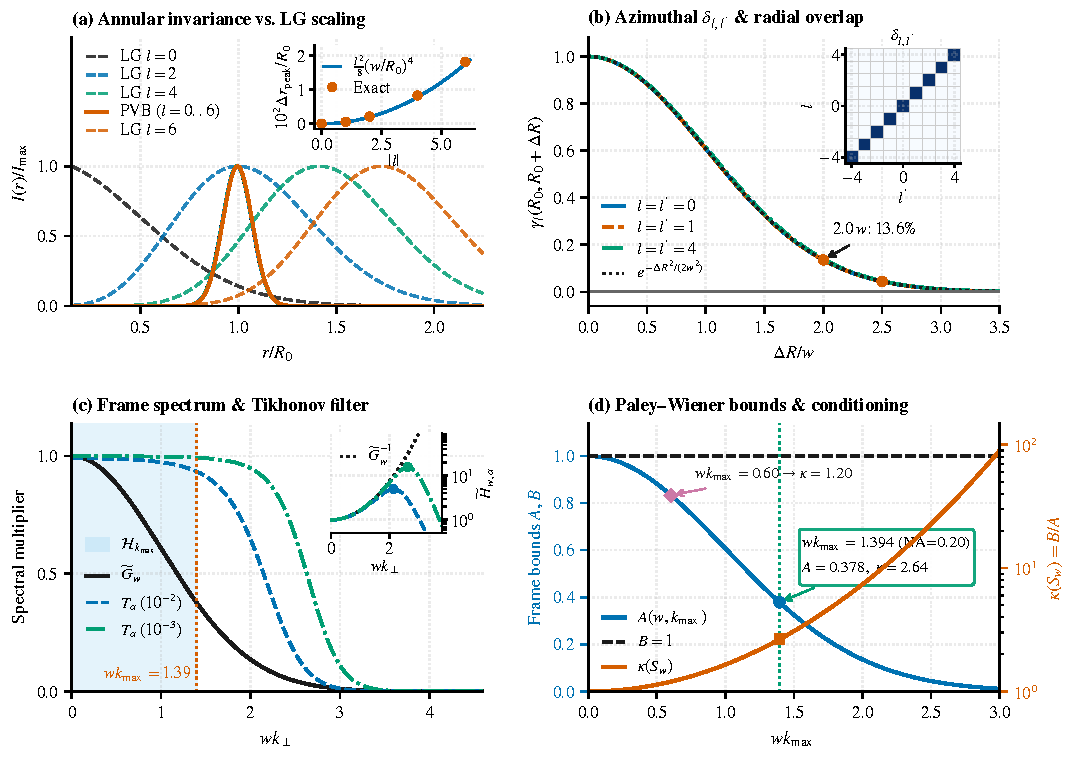
\includegraphics[width=0.82\textwidth]{figures/fig1_frame_spectrum.pdf}
\caption{Physical PVB continuous frame structure and spectral bounds. (a) Peak-normalized radial intensity $I(r)/I_{\max}$ for physical PVBs ($w/R_0 = 0.15$, solid) across $l = 0,2,4,6$ versus $\mathrm{LG}_{0,l}$ ($w_0 = R_0$, dashed); inset compares the exact transcendental differential shift $\Delta r_{\mathrm{peak}}(l)/R_0$ ($w/R_0 = 0.25$, circles) against $(l^2/8)(w/R_0)^4$ [Eq.~\eqref{eq:peak_shift}]. (b) Unit-normalized radial overlap $\gamma_l(R_0, R_0+\Delta R)$ [Eq.~\eqref{eq:gamma_normalized}] at $R_0 = 4w$ for $l = 0,1,4$ versus the $l$-independent Gaussian asymptote $e^{-\Delta R^2/(2w^2)}$ (dotted), marking $13.6\%$ at $\Delta R = 2.0\,w$ and $4.40\%$ at $\Delta R = 2.5\,w$; inset confirms azimuthal Kronecker orthogonality $\delta_{l,l'}$. (c) Continuous-frame Fourier multiplier $\widetilde{G}_w(k_\perp)$ and Tikhonov transfer $T_{\alpha_{\mathrm{reg}}}(k_\perp)$ ($\alpha_{\mathrm{reg}} = 10^{-2}, 10^{-3}$) with Paley--Wiener passband $\mathcal{H}_{k_{\max}}$ shaded up to $w k_{\max} = 1.394$; inset shows the deconvolution noise gain $\widetilde{H}_{w,\alpha_{\mathrm{reg}}}(k_\perp)$ peaking at $(2\sqrt{\alpha_{\mathrm{reg}}})^{-1}$. (d) Sharp Paley--Wiener bounds $A(w,k_{\max}), B = 1$ and condition number $\kappa(S_{w,k_{\max}})$ versus $w k_{\max}$, annotating both the low-NA reference ($w k_{\max} = 0.604 \implies A = 0.833, \kappa = 1.20$) and the telecom RCF benchmark ($\lambda = 1550\,\mathrm{nm}, \mathrm{NA} = 0.20, w = 1.72\,\mu\mathrm{m}$: $w k_{\max} = 1.394 \implies A = 0.378, \kappa = 2.64$).}
\label{fig:frame_spectrum}
\end{figure*}

\subsection{Continuous Frame Operator, Bessel Bound, and Convolution Kernel}
\label{subsec:frame_operator}

A family $\{\Phi_\omega\}_{\omega\in\Omega}$ in a separable Hilbert space $\mathcal{H}$ equipped with $\sigma$-finite measure $\mu$ forms a continuous Hilbert frame~\cite{Duffin1952,Daubechies1990,Ali1993,Christensen2016} if $\omega \mapsto \braket{\Phi_\omega}{\psi}$ is measurable and there exist constants $0 < A \le B < \infty$ such that for all $\psi \in \mathcal{H}$,
\begin{equation}
A \norm{\psi}_{\mathcal{H}}^2 \le \int_\Omega \abs{\braket{\Phi_\omega}{\psi}}^2\,d\mu(\omega) \le B \norm{\psi}_{\mathcal{H}}^2.
\label{eq:frame_def}
\end{equation}
If only the upper inequality holds ($B < \infty$), $\{\Phi_\omega\}$ is a continuous Bessel family. With index space $\Omega = \mathbb{Z} \times (0,\infty)$, product measure $d\mu(l,R) = R\,dR$, and analysis operator $(T\psi)(l,R) = \braket{\Phi_{l,R}}{\psi}$, the PVB frame operator $S_w = T^* T : \mathcal{H} \to \mathcal{H}$ is defined weakly by
\begin{equation}
S_w\psi = \sum_{l\in\mathbb{Z}} \int_0^\infty R\,dR\, \braket{\Phi_{l,R}}{\psi}\Phi_{l,R}.
\label{eq:frame_op}
\end{equation}
We adopt the non-unitary 2D spatial Fourier transform convention
\begin{align}
\widetilde{\psi}(\mathbf{k}) &= \int_{\mathbb{R}^2} \psi(\mathbf{r}) e^{-i\mathbf{k}\cdot\mathbf{r}}\,d^2\mathbf{r}, \nonumber \\
\psi(\mathbf{r}) &= \int_{\mathbb{R}^2} \widetilde{\psi}(\mathbf{k}) e^{i\mathbf{k}\cdot\mathbf{r}}\,\frac{d^2\mathbf{k}}{(2\pi)^2},
\label{eq:ft_convention}
\end{align}
with radial spatial frequency $k_\perp = \abs{\mathbf{k}} = \sqrt{k_x^2 + k_y^2}$ and Plancherel identity $\braket{\phi}{\psi}_{L^2} = (2\pi)^{-2}\braket{\widetilde{\phi}}{\widetilde{\psi}}_{L^2}$.

\begin{lemma}[Continuous Bessel upper bound $B=1$]
\label{lem:bessel_upper}
Under the scaling $C_0$ of Eq.~\eqref{eq:C0_norm} and measure $d\mu(l,R) = R\,dR$, the physical PVB family $\{\Phi_{l,R}\}_{l\in\mathbb{Z},\,R>0}$ satisfies for every $\psi \in L^2(\mathbb{R}^2)$
\begin{equation}
\norm{T\psi}_{L^2(\Omega,\mu)}^2 = \int_{\mathbb{R}^2} e^{-w^2 k_\perp^2/2}\abs{\widetilde{\psi}(\mathbf{k})}^2\,\frac{d^2\mathbf{k}}{(2\pi)^2} \le \norm{\psi}_{L^2}^2,
\label{eq:bessel_lemma}
\end{equation}
establishing that $\{\Phi_{l,R}\}$ is a continuous Bessel system on $L^2(\mathbb{R}^2)$ with upper bound $B = 1$.
\end{lemma}
\begin{proof}
Expanding $e^{-i\mathbf{k}\cdot\mathbf{r}}$ via the Jacobi--Anger identity and evaluating the radial integral by analytic continuation of Eq.~\eqref{eq:weber_identity} (Gradshteyn--Ryzhik formula 6.631.4~\cite{Gradshteyn2014}), the 2D Fourier transform~\eqref{eq:ft_convention} of Eq.~\eqref{eq:pvb_mode} is
\begin{equation}
\widetilde{\Phi}_{l,R}(\mathbf{k}) = \sqrt{2\pi}\,(-i)^{\abs{l}} e^{il\phi_k} \exp\!\left(-\frac{w^2 k_\perp^2}{4}\right) J_{\abs{l}}(R k_\perp).
\label{eq:pvb_ft}
\end{equation}
Decomposing $\widetilde{\psi}(k_\perp,\phi_k) = \sum_{l\in\mathbb{Z}} \widetilde{\psi}_l(k_\perp)e^{il\phi_k}$ in polar Fourier coordinates, Plancherel's identity gives $(T\psi)(l,R) = \braket{\Phi_{l,R}}{\psi} = (2\pi)^{-1/2} i^{\abs{l}} \allowbreak \int_0^\infty k_\perp\,dk_\perp\, \allowbreak e^{-w^2 k_\perp^2/4}\widetilde{\psi}_l(k_\perp) J_{\abs{l}}(Rk_\perp)$, which is $(2\pi)^{-1/2} i^{\abs{l}}$ times the order-$\abs{l}$ Hankel transform of $e^{-w^2 k_\perp^2/4}\widetilde{\psi}_l(k_\perp)$. Because the Hankel transform is unitary on $L^2((0,\infty), R\,dR)$, integrating $\abs{(T\psi)(l,R)}^2 R\,dR$ over $R \in (0,\infty)$ and summing over $l \in \mathbb{Z}$ yields
\begin{align*}
\norm{T\psi}_{L^2(\Omega,\mu)}^2 &= \frac{1}{2\pi}\sum_{l\in\mathbb{Z}} \int_0^\infty k_\perp\,dk_\perp\,e^{-w^2 k_\perp^2/2}\abs{\widetilde{\psi}_l(k_\perp)}^2 \\
&= \int_{\mathbb{R}^2} e^{-w^2 k_\perp^2/2}\abs{\widetilde{\psi}(\mathbf{k})}^2\,\frac{d^2\mathbf{k}}{(2\pi)^2}.
\end{align*}
Since $0 < e^{-w^2 k_\perp^2/2} \le 1$ for all $k_\perp \ge 0$, Parseval's identity gives $\norm{T\psi}_{L^2(\Omega,\mu)}^2 \le (2\pi)^{-2}\norm{\widetilde{\psi}}_{L^2}^2 = \norm{\psi}_{L^2}^2$.
\end{proof}

\begin{proposition}[Azimuthal--radial decoupling and Gaussian convolution kernel]
\label{prop:conv_kernel}
For any $w > 0$, the PVB family $\{\Phi_{l,R}\}_{l\in\mathbb{Z},\,R>0}$ obeys Eq.~\eqref{eq:overlap_closed}, and its frame operator~\eqref{eq:frame_op} acts on $L^2(\mathbb{R}^2)$ as the self-adjoint isotropic Gaussian convolution $(S_w\psi)(\mathbf{r}) = (G_w * \psi)(\mathbf{r})$ with kernel $G_w(\mathbf{r}) = (2\pi w^2)^{-1}\exp(-\abs{\mathbf{r}}^2/(2w^2))$, diagonalized in Fourier space as
\begin{equation}
\widetilde{(S_w\psi)}(\mathbf{k}) = \widetilde{G}_w(k_\perp)\widetilde{\psi}(\mathbf{k}), \quad \widetilde{G}_w(k_\perp) = e^{-w^2 k_\perp^2/2}.
\label{eq:fourier_diag}
\end{equation}
\end{proposition}
\begin{proof}
By polarization of Eq.~\eqref{eq:bessel_lemma} in Lemma~\ref{lem:bessel_upper}, for any $\phi,\psi \in L^2(\mathbb{R}^2)$ we have $\braket{\phi}{S_w\psi} = \braket{T\phi}{T\psi}_{L^2(\Omega,\mu)} = (2\pi)^{-2}\int_{\mathbb{R}^2} e^{-w^2 k_\perp^2/2}\widetilde{\phi}^*(\mathbf{k})\widetilde{\psi}(\mathbf{k})\,d^2\mathbf{k}$, which proves Eq.~\eqref{eq:fourier_diag}. Inverse Fourier transformation via Eq.~\eqref{eq:ft_convention} yields $(S_w\psi)(\mathbf{r}) = (G_w * \psi)(\mathbf{r})$ with $G_w(\mathbf{r}) = (2\pi w^2)^{-1}e^{-\abs{\mathbf{r}}^2/(2w^2)}$, recovering in exact operator form the Gaussian smoothing action noted in Appendix~D of Ref.~\cite{Ferreira2026}.
\end{proof}

\subsection{Paley--Wiener Stability Bounds and Physical Obstructions to \texorpdfstring{$w \to 0$}{w -> 0}}
\label{subsec:paley_wiener}

Real paraxial optical setups transmit transverse spatial frequencies bounded by the collection cutoff $k_{\max} = k_0 \mathrm{NA}$. Introducing the Paley--Wiener bandlimited Hilbert space
\begin{align}
\mathcal{H}_{k_{\max}} &= \left\{\psi \in L^2(\mathbb{R}^2) : \operatorname{supp}(\widetilde{\psi}) \subseteq \{\abs{\mathbf{k}} \le k_{\max}\}\right\} \nonumber \\
&= \bigoplus_{l\in\mathbb{Z}} \mathcal{H}_{l,k_{\max}},
\label{eq:paley_wiener}
\end{align}
and its orthogonal Fourier-cutoff projector $P_{k_{\max}}\psi = \mathcal{F}^{-1}\{\mathbf{1}_{\{k_\perp \le k_{\max}\}}\widetilde{\psi}\}$, Lemma~\ref{lem:bessel_upper} and Proposition~\ref{prop:conv_kernel} yield our sharp stability theorem.

\begin{theorem}[Paley--Wiener frame stability and projected canonical dual]
\label{thm:pw_bounds}
(i) On unconstrained $L^2(\mathbb{R}^2)$, $\{\Phi_{l,R}\}$ is a continuous Bessel family with optimal upper bound $B = 1$ and vanishing lower bound $A = \inf_{k_\perp \ge 0} \widetilde{G}_w(k_\perp) = 0$; consequently, $S_w^{-1}$ is unbounded on $L^2(\mathbb{R}^2)$ and $S_w^{-1}\Phi_{l,R} \notin L^2(\mathbb{R}^2)$. (ii) Restricted to $\mathcal{H}_{k_{\max}}$ of Eq.~\eqref{eq:paley_wiener} ($0 < k_{\max} < \infty$), the projected family $\{P_{k_{\max}}\Phi_{l,R}\}$ forms a continuous Hilbert frame satisfying Eq.~\eqref{eq:frame_def} with restricted frame operator $S_{w,k_{\max}} = P_{k_{\max}} S_w P_{k_{\max}}\big|_{\mathcal{H}_{k_{\max}}}$, sharp frame bounds
\begin{equation}
A(w, k_{\max}) = \exp\!\left(-\frac{w^2 k_{\max}^2}{2}\right) > 0, \qquad B = 1,
\label{eq:optimal_bounds}
\end{equation}
spectral condition number $\kappa(S_{w,k_{\max}}) = B/A = \exp(w^2 k_{\max}^2/2) < \infty$, and bounded canonical dual frame elements $\widetilde{\Phi}_{l,R} = S_{w,k_{\max}}^{-1} P_{k_{\max}}\Phi_{l,R} \in \mathcal{H}_{k_{\max}}$.
\end{theorem}
\begin{proof}
For any $\psi \in \mathcal{H}_{k_{\max}}$, $P_{k_{\max}}\psi = \psi$, so $\braket{P_{k_{\max}}\Phi_{l,R}}{\psi} = \braket{\Phi_{l,R}}{\psi}$. By Lemma~\ref{lem:bessel_upper}, $\norm{T\psi}_{L^2(\Omega,\mu)}^2 = \braket{\psi}{S_w\psi} \le \norm{\psi}_{L^2}^2$, giving $B \le 1$, while $\widetilde{G}_w(k_\perp) \ge e^{-w^2 k_{\max}^2/2}$ for all $k_\perp \in [0, k_{\max}]$ gives $\braket{\psi}{S_{w,k_{\max}}\psi} \ge e^{-w^2 k_{\max}^2/2}\norm{\psi}_{L^2}^2$.

To prove sharpness of both constants in Eq.~\eqref{eq:optimal_bounds}, define for $\epsilon \in (0, k_{\max})$ the explicit unit-$L^2(\mathbb{R}^2)$-normalized Fourier-annulus test families in $\mathcal{H}_{k_{\max}}$ [accounting for the $(2\pi)^{-2}$ Plancherel prefactor of Eq.~\eqref{eq:ft_convention}]:
\begin{align}
\widetilde{\psi}_\epsilon^{(+)}(\mathbf{k}) &= \frac{2\pi}{\sqrt{\pi\epsilon^2}}\,\mathbf{1}_{\{0 < k_\perp \le \epsilon\}}(\mathbf{k}), \nonumber \\
\widetilde{\psi}_\epsilon^{(-)}(\mathbf{k}) &= \frac{2\pi}{\sqrt{\pi\epsilon(2k_{\max}-\epsilon)}}\,\mathbf{1}_{\{k_{\max}-\epsilon \le k_\perp \le k_{\max}\}}(\mathbf{k}),
\label{eq:test_annuli}
\end{align}
where $\pi\epsilon(2k_{\max}-\epsilon) \sim 2\pi k_{\max}\epsilon$ as $\epsilon \to 0^+$ and $\norm{\psi_\epsilon^{(\pm)}}_{L^2}^2 = 1$. Direct radial integration of Eq.~\eqref{eq:bessel_lemma} for Eq.~\eqref{eq:test_annuli} yields in closed form
\begin{align}
\braket{\psi_\epsilon^{(+)}}{S_w\psi_\epsilon^{(+)}} &= \frac{2\left(1 - e^{-w^2\epsilon^2/2}\right)}{w^2\epsilon^2} \xrightarrow[\epsilon \to 0^+]{} 1 = B, \nonumber \\
\braket{\psi_\epsilon^{(-)}}{S_w\psi_\epsilon^{(-)}} &= \frac{2\left[e^{-w^2(k_{\max}-\epsilon)^2/2} - e^{-w^2 k_{\max}^2/2}\right]}{w^2\epsilon(2k_{\max}-\epsilon)} \nonumber \\
&\xrightarrow[\epsilon \to 0^+]{} e^{-w^2 k_{\max}^2/2} = A(w, k_{\max}).
\label{eq:sharpness_limits}
\end{align}
Sending $k_{\max} \to \infty$ in Eq.~\eqref{eq:sharpness_limits} proves $\inf_{\norm{\psi}=1}\braket{\psi}{S_w\psi} = 0$ on $L^2(\mathbb{R}^2)$. Finally, because $\widetilde{\Phi}_{l,R}(\mathbf{k})$ in Eq.~\eqref{eq:pvb_ft} has unbounded spatial-frequency support, $\Phi_{l,R} \notin \mathcal{H}_{k_{\max}}$ and $e^{+w^2 k_\perp^2/2}\widetilde{\Phi}_{l,R}(\mathbf{k}) \propto e^{+w^2 k_\perp^2/4} J_{\abs{l}}(Rk_\perp) \notin L^2(\mathbb{R}^2)$, so $S_w^{-1}\Phi_{l,R} \notin L^2(\mathbb{R}^2)$, whereas on $\mathcal{H}_{k_{\max}}$ the restricted multiplier $e^{+w^2 k_\perp^2/2}\mathbf{1}_{\{k_\perp \le k_{\max}\}}$ is bounded by $A^{-1} = e^{w^2 k_{\max}^2/2}$ (and $S_{w,k_{\max}}^{-1/2}$ by $A^{-1/2}$), guaranteeing $\widetilde{\Phi}_{l,R} \in \mathcal{H}_{k_{\max}}$.
\end{proof}

Notice that $\mathcal{H}_{k_{\max}}$ is a reproducing-kernel Hilbert space (RKHS)~\cite{PaulsenRaghupathi2016} with bandlimited Airy--Bessel reproducing kernel, and that fundamental wave physics forbids taking the singular Dirac limit $w \to 0$: (i) transverse wavevector variance diverges as $\langle k_\perp^2 \rangle \sim w^{-2} \to \infty$, breaking paraxial electrodynamics and converting high-$k_\perp$ tails into evanescent waves above $k_0$; (ii) beam propagation quality degrades as $M^2 \sim R/w \to \infty$; (iii) any finite lens aperture $D$ enforces the diffraction lower bound $w \ge 2\lambda f/(\pi D)$ while fixed optical power $P$ drives peak ring irradiance as $I_{\max} \propto (R w)^{-1}$; and (iv) $\Phi_{l,R}^{\mathrm{ideal}} \notin L^2(\mathbb{R}^2)$ belongs strictly to the distributional dual $\Phi^\times$ of a Gel'fand rigged Hilbert triplet $\Phi \subset L^2(\mathbb{R}^2) \subset \Phi^\times$~\cite{Gelfand1964}. Table~\ref{tab:frame_comparison} synthesizes the structural hierarchy comparing Dirac PVBs, physical PVBs, orthogonal $\mathrm{LG}_{p,l}$ modes, and Glauber coherent states $\ket{\alpha}$~\cite{Klauder1985,Perelomov1986,Gazeau2009}.

\begin{table*}[t]
\caption{Structural comparison of ideal Dirac PVBs, physical finite-width PVBs, Laguerre--Gaussian ($\mathrm{LG}_{p,l}$) eigenmodes, and Glauber coherent states across function space, orthogonality, frame bounds, canonical duals, and optical pupil footprint. At the radial endpoint $R = 0$, $\Phi_{l,0} \equiv 0$ ($l \neq 0$) and $\Phi_{0,0}(r) = C_0 e^{-r^2/w^2}$ carries zero $R\,dR$ measure.}
\label{tab:frame_comparison}
\begin{ruledtabular}
\footnotesize
\begin{tabular}{p{2.2cm}p{3.6cm}p{4.3cm}p{3.2cm}p{3.3cm}}
Property & Ideal Dirac PVB ($w=0$) & Physical PVB ($w>0$) & $\mathrm{LG}_{p,l}$ Modes & Coherent States $\ket{\alpha}$ \\
\hline
Function space & Rigged dual $\Phi^\times$ ($\notin L^2$) & $L^2(\mathbb{R}^2)$ (frame on $\mathcal{H}_{k_{\max}}$) & $L^2(\mathbb{R}^2)$ (complete ONB) & Bargmann--Fock $L^2$ \\
Orthogonality & $\delta_{l,l'}\delta(R-R')/R$ & $\delta_{l,l'}$ in $l$; $\gamma_l(R,R') > 0$ in $R$ & $\delta_{p,p'}\delta_{l,l'}$ (orthogonal) & $\abs{\braket{\alpha}{\beta}} = e^{-\abs{\alpha-\beta}^2/2}$ \\
Completeness / bounds & Generalized ONB & $A = e^{-w^2 k_{\max}^2/2},\, B = 1$ ($\mathcal{H}_{k_{\max}}$) & Tight ($A = B = 1$) & Tight ($A = B = 1$, measure $d^2\alpha/\pi$) \\
Dual / inversion & Self-dual ($\notin L^2$) & $S_w = G_w * \cdot$; projected / Tikhonov dual & Self-dual ($S = \mathbb{I}$) & Self-dual ($S = \mathbb{I}$) \\
Pupil / RCF footprint & Singular (infinite $k_\perp$ variance) & $l$-invariant ring $R$ ($\bar{\eta}_l = 98.5\%$ in RCF) & $r_{\mathrm{rms}} = w_0\sqrt{2p+\abs{l}+1}$ ($l$-clipping) & Displaced phase-space packet \\
\end{tabular}
\end{ruledtabular}
\end{table*}

\section{Core Analytical Properties of the Overcomplete PVB Frame}
\label{sec:properties}

\subsection{Projected and Tikhonov-Regularized Canonical Dual Frames}
\label{subsec:tikhonov_dual}

When reconstructing an optical field from noisy frame measurements, $\psi_{\mathrm{meas}}(\mathbf{r}) = (S_w\psi)(\mathbf{r}) + \varepsilon(\mathbf{r})$ with additive noise field $\varepsilon(\mathbf{r})$, applying the unregularized inverse multiplier $\widetilde{G}_w^{-1}(k_\perp) = \exp(+w^2 k_\perp^2/2)$ amplifies high-$k_\perp$ noise components $\widetilde{\varepsilon}(\mathbf{k})$ exponentially when $w k_{\max} \gtrsim 1$. To stabilize inversion over $\mathcal{H} \in \{L^2(\mathbb{R}^2), \mathcal{H}_{k_{\max}}\}$, we solve the Tikhonov variational problem with dimensionless regularization weight $\alpha_{\mathrm{reg}} > 0$:
\begin{equation}
\min_{\psi \in \mathcal{H}} \left\{ \norm{S_w\psi - \psi_{\mathrm{meas}}}_{L^2}^2 + \alpha_{\mathrm{reg}}\norm{\psi}_{L^2}^2 \right\}.
\label{eq:tikhonov_opt}
\end{equation}

\begin{proposition}[Tikhonov-regularized dual frame and noise-gain peak]
\label{prop:tikhonov_dual}
For every $\alpha_{\mathrm{reg}} > 0$, the unique minimizer of Eq.~\eqref{eq:tikhonov_opt} defines the bounded operator $S_{w,\alpha_{\mathrm{reg}}}^{-1} = (S_w^2 + \alpha_{\mathrm{reg}}\mathbb{I})^{-1}S_w$, regularized dual vectors $\widetilde{\Phi}_{l,R}^{(\alpha_{\mathrm{reg}})} = S_{w,\alpha_{\mathrm{reg}}}^{-1}\Phi_{l,R} \in L^2(\mathbb{R}^2)$ (or $P_{k_{\max}}S_{w,\alpha_{\mathrm{reg}}}^{-1}P_{k_{\max}}\Phi_{l,R} \in \mathcal{H}_{k_{\max}}$), and spectral deconvolution
\begin{equation}
\widetilde{(S_{w,\alpha_{\mathrm{reg}}}^{-1}\psi_{\mathrm{meas}})}(\mathbf{k}) = T_{\alpha_{\mathrm{reg}}}(k_\perp)\widetilde{\psi}(\mathbf{k}) + \widetilde{H}_{w,\alpha_{\mathrm{reg}}}(k_\perp)\widetilde{\varepsilon}(\mathbf{k}),
\label{eq:synth_multiplier}
\end{equation}
where $T_{\alpha_{\mathrm{reg}}}(k_\perp) = \widetilde{G}_w^2(k_\perp)/[\widetilde{G}_w^2(k_\perp) + \alpha_{\mathrm{reg}}] < 1$ is the signal shrinkage transfer and
\begin{equation}
\widetilde{H}_{w,\alpha_{\mathrm{reg}}}(k_\perp) = \frac{\widetilde{G}_w(k_\perp)}{\widetilde{G}_w^2(k_\perp) + \alpha_{\mathrm{reg}}} = \frac{e^{-w^2 k_\perp^2/2}}{e^{-w^2 k_\perp^2} + \alpha_{\mathrm{reg}}}.
\label{eq:tikhonov_filter}
\end{equation}
For $\alpha_{\mathrm{reg}} \in (0,1)$, $\widetilde{H}_{w,\alpha_{\mathrm{reg}}}(k_\perp)$ attains its global maximum $\widetilde{H}_{\max} = (2\sqrt{\alpha_{\mathrm{reg}}})^{-1}$ at $k_{\mathrm{peak}} = w^{-1}\sqrt{\ln(1/\alpha_{\mathrm{reg}})}$ and decays exponentially as $\alpha_{\mathrm{reg}}^{-1}e^{-w^2 k_\perp^2/2}$ only for $k_\perp \gg k_{\mathrm{peak}}$.
\end{proposition}
\begin{proof}
Taking the Fr\'echet derivative of Eq.~\eqref{eq:tikhonov_opt} in Fourier space gives $[\widetilde{G}_w^2(k_\perp) + \alpha_{\mathrm{reg}}]\widetilde{\psi}(\mathbf{k}) = \widetilde{G}_w(k_\perp)\widetilde{\psi}_{\mathrm{meas}}(\mathbf{k})$, establishing Eqs.~\eqref{eq:synth_multiplier}--\eqref{eq:tikhonov_filter}. Writing $\widetilde{H}_{w,\alpha_{\mathrm{reg}}} = (g + \alpha_{\mathrm{reg}}/g)^{-1}$ with $g = \widetilde{G}_w(k_\perp) \in (0,1]$, the arithmetic--geometric mean inequality $g + \alpha_{\mathrm{reg}}/g \ge 2\sqrt{\alpha_{\mathrm{reg}}}$ is saturated uniquely at $g = \sqrt{\alpha_{\mathrm{reg}}}$, i.e., $k_{\mathrm{peak}} = w^{-1}\sqrt{\ln(1/\alpha_{\mathrm{reg}})}$.
\end{proof}

Crucially, contrary to naive intuition that deconvolution roll-off begins near $1/w$, for $\alpha_{\mathrm{reg}} = 10^{-4}$ and $w = 0.5\,\ell_0$ the noise gain rises to $\widetilde{H}_{\max} = 50.0$ at $k_{\mathrm{peak}} = 6.070\,\ell_0^{-1} \gg 1/w = 2.0\,\ell_0^{-1}$ [Fig.~\ref{fig:frame_spectrum}(c) inset]. Moreover, because $T_{\alpha_{\mathrm{reg}}}(k_\perp) < 1$ strictly for every $\alpha_{\mathrm{reg}} > 0$, regularized inversion trades controlled shrinkage bias for dramatic variance suppression; zero-bias reconstruction holds exclusively at $\alpha_{\mathrm{reg}} = 0$ on $\mathcal{H}_{k_{\max}}$ via Theorem~\ref{thm:pw_bounds}.

\begin{figure*}[t]
\centering
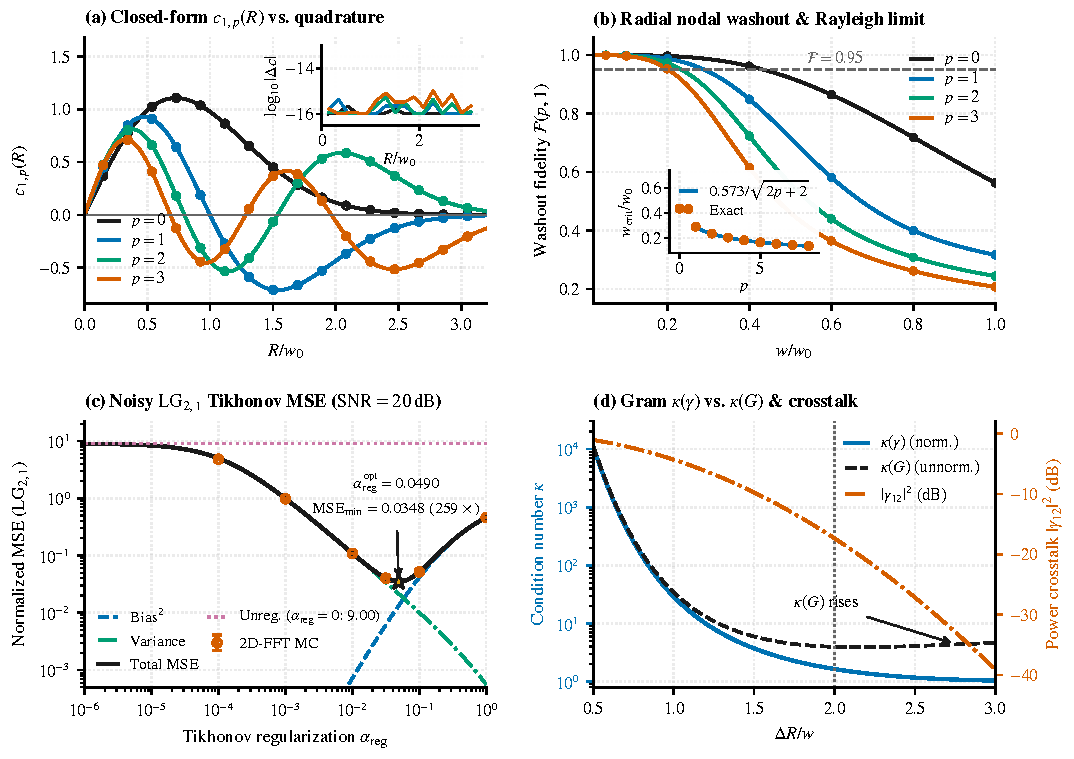
\includegraphics[width=0.82\textwidth]{figures/fig2_laguerre_regularization.pdf}
\caption{Laguerre--Gaussian expansion, radial washout, regularized noisy reconstruction, and discrete Gram conditioning. (a) Closed-form coefficients $c_{1,p}(R)$ [Eq.~\eqref{eq:c_lp_exact}, solid] versus adaptive quadrature (circles) for $\mathrm{LG}_{p,1}$ ($p = 0\text{--}3$, $w/w_0 = 0.25$); inset shows $\log_{10}\abs{\Delta c} < -14$. (b) Nodal washout fidelity $\mathcal{F}(p,1,w/w_0)$ [Eq.~\eqref{eq:fidelity_fourier}] with Table~\ref{tab:fidelity} values (dots); inset compares exact $\mathcal{F} = 0.95$ roots $w_{\mathrm{crit}}/w_0$ ($p = 0\text{--}8$) against $0.573/\sqrt{2p+\abs{l}+1}$ ($l = 1$). (c) Noisy $\mathrm{LG}_{2,1}$ reconstruction error ($w/w_0 = 0.25$, $w k_{\max} = 3.0$, bandlimited white noise power $P_\varepsilon = 0.01$, input $\mathrm{SNR} = 20\,\mathrm{dB}$) decomposed into analytical $\mathrm{Bias}^2$ and variance alongside $256\times 256$ 2D-FFT Monte Carlo trials (circles, $\pm 1\,\mathrm{SEM}$), reducing unregularized error $\mathrm{MSE}(\alpha_{\mathrm{reg}} = 0) = 9.002$ to $\mathrm{MSE}_{\min} = 0.03481$ at $\alpha_{\mathrm{reg}}^{\mathrm{opt}} = 0.04902$ ($258.6\times$ suppression). (d) Monotonic unit-normalized $\kappa(\gamma)$ versus diverging unnormalized $\kappa(G)$ (left axis) and adjacent power crosstalk $\abs{\gamma_{12}}^2$ in dB (right axis) for Table~\ref{tab:gram_matrix}.}
\label{fig:laguerre_regularization}
\end{figure*}

\subsection{Exact Closed-Form Expansion of \texorpdfstring{$\mathrm{LG}_{p,l}$}{LG\_\{p,l\}} Modes (\texorpdfstring{$p \ge 0$}{p >= 0})}
\label{subsec:analytic_lg_expansion}

Consider an arbitrary unit-$L^2$-normalized Laguerre--Gaussian eigenmode $\mathrm{LG}_{p,l}$ of waist $w_0$ ($p \in \mathbb{Z}_{\ge 0}$, $l \in \mathbb{Z}$),
\begin{equation}
\psi_{p,l}(r,\phi) = N_{p,l}\!\left(\frac{\sqrt{2}\,r}{w_0}\right)^{\abs{l}} L_p^{\abs{l}}\!\left(\frac{2r^2}{w_0^2}\right) e^{-r^2/w_0^2 + il\phi},
\label{eq:lg_def}
\end{equation}
with $N_{p,l} = \sqrt{2p!/[\pi(p+\abs{l})!]}/w_0$ and continuous PVB frame analysis coefficients $c_{l,p}(R) = \braket{\Phi_{l,R}}{\psi_{p,l}}$. Extending the $p = 0$ calculation of Ref.~\cite{Ferreira2026} to all radial orders $p \ge 0$, we obtain an exact finite algebraic expansion.

\begin{theorem}[Exact closed-form expansion of $\mathrm{LG}_{p,l}$ modes]
\label{thm:c_lp_exact}
For all $p \in \mathbb{Z}_{\ge 0}$, $l \in \mathbb{Z}$, $w > 0$, and $w_0 > 0$, the continuous PVB projection $c_{l,p}(R) = \braket{\Phi_{l,R}}{\psi_{p,l}}$ is given exactly by the $(p+1)$-term finite sum
\begin{equation}
c_{l,p}(R) = \mathcal{A}_{p,l}(R) \sum_{m=0}^p (-1)^m \binom{p+\abs{l}}{p-m} \xi^m L_m^{\abs{l}}(-\zeta_R),
\label{eq:c_lp_exact}
\end{equation}
with dimensionless width parameter and Laguerre argument
\begin{equation}
\xi = \frac{2w^2}{w_0^2 + w^2}, \qquad \zeta_R = \frac{R^2 w_0^2}{w^2(w_0^2 + w^2)},
\label{eq:xi_zeta_defs}
\end{equation}
and envelope prefactor
\begin{equation}
\mathcal{A}_{p,l}(R) = 2^{\frac{\abs{l}}{2}+1}\sqrt{\frac{p!}{(p+\abs{l})!}}\,\frac{R^{\abs{l}} w_0^{\abs{l}+1}}{(w_0^2 + w^2)^{\abs{l}+1}} \exp\!\left(-\frac{R^2}{w_0^2 + w^2}\right).
\label{eq:A_prefactor}
\end{equation}
These coefficients synthesize the frame-smoothed $\mathrm{LG}_{p,l}$ mode identically via
\begin{equation}
(S_w\psi_{p,l})(\mathbf{r}) = \int_0^\infty R\,dR\, c_{l,p}(R)\,\Phi_{l,R}(\mathbf{r}).
\label{eq:frame_synthesis_lg}
\end{equation}
\end{theorem}

The complete proof—combining the finite Laguerre polynomial expansion, Gradshteyn--Ryzhik formula 6.631.1~\cite{Gradshteyn2014}, and Kummer's confluent hypergeometric transformation—together with explicit $p = 0$ Weber verification and a 60-point quadrature benchmark ($\abs{\Delta c} \le 1.51\times 10^{-15}$, $\abs{\Delta c}/\abs{c} \le 3.64\times 10^{-12}$) is given in Appendix~\ref{app:lg_expansion} [Fig.~\ref{fig:laguerre_regularization}(a)]. Computationally, Eq.~\eqref{eq:c_lp_exact} reduces highly oscillatory 2D Bessel--Laguerre overlap integrals to an $\mathcal{O}(p)$ finite algebraic polynomial evaluation (via three-term Laguerre recurrence), providing an orders-of-magnitude speedup for real-time modal decomposition and multi-plane tomography.

\subsection{Radial Resolution Limits and Nodal Washout}
\label{subsec:nodal_washout}

Because $\psi_{p,l}$ exhibits $p$ concentric radial phase-flip nodes~\cite{Allen1992,Siegman1986,Walborn2010}, Gaussian convolution by $S_w$ washes out fine radial structure once $w$ approaches the nodal spacing. Using Eq.~\eqref{eq:fourier_diag} with $u = w_0^2 k_\perp^2/2$, $a = w^2/w_0^2$, and normalized spectral density $\rho_{p,l}(u) = [p!/(p+\abs{l})!]u^{\abs{l}} e^{-u}[L_p^{\abs{l}}(u)]^2$, the uncompensated frame fidelity $\mathcal{F}(p,l,w/w_0) = \abs{\braket{\psi_{p,l}}{S_w\psi_{p,l}}}^2/\norm{S_w\psi_{p,l}}_{L^2}^2$ reduces to
\begin{equation}
\mathcal{F}(p,l,w/w_0) = \frac{\left(\int_0^\infty e^{-au}\,\rho_{p,l}(u)\,du\right)^2}{\int_0^\infty e^{-2au}\,\rho_{p,l}(u)\,du}.
\label{eq:fidelity_fourier}
\end{equation}
Table~\ref{tab:fidelity} reports exact values of Eq.~\eqref{eq:fidelity_fourier} at $l = 1$; notably, at $w/w_0 = 1.00$ they coincide with the exact rational fractions $9/16$, $81/256$, $18225/74752$, and $8037225/38862848$ for $p = 0,1,2,3$.

\begin{table}[t]
\caption{Exact radial reconstruction fidelity $\mathcal{F}(p, l=1, w/w_0)$ of $\mathrm{LG}_{p,1}$ modes under the PVB frame operator $S_w$ across relative ring half-widths $w/w_0$. At $w/w_0 = 1.00$, entries match the exact rationals $9/16$, $81/256$, $18225/74752$, and $8037225/38862848$.}
\label{tab:fidelity}
\begin{ruledtabular}
\setlength{\tabcolsep}{4pt}
\begin{tabular}{ccccc}
$w / w_0$ & $\mathcal{F}(p=0)$ & $\mathcal{F}(p=1)$ & $\mathcal{F}(p=2)$ & $\mathcal{F}(p=3)$ \\
\hline
0.05 & 0.99999 & 0.99995 & 0.99989 & 0.99980 \\
0.10 & 0.99980 & 0.99921 & 0.99822 & 0.99683 \\
0.20 & 0.99704 & 0.98782 & 0.97282 & 0.95276 \\
0.40 & 0.96231 & 0.84935 & 0.72301 & 0.61610 \\
0.60 & 0.86477 & 0.58216 & 0.43953 & 0.36419 \\
0.80 & 0.71861 & 0.39960 & 0.30831 & 0.26129 \\
1.00 & 0.56250 & 0.31641 & 0.24381 & 0.20681 \\
\end{tabular}
\end{ruledtabular}
\end{table}

\begin{corollary}[Generalized radial Rayleigh criterion]
\label{cor:rayleigh_radial}
Maintaining reconstruction fidelity $\mathcal{F}(p,l,w/w_0) \ge 0.95$ requires: (i) for $p = 0$, with $q_l \equiv 0.95^{1/(\abs{l}+1)}$, the exact closed-form threshold
\begin{equation}
w \le w_{\mathrm{crit}}(0,l) = w_0 \left[\left(1 - \sqrt{1 - q_l}\right)^{-1} - 1\right]^{1/2},
\label{eq:rayleigh_p0}
\end{equation}
yielding $0.5367\,w_0$ ($l = 0$), $0.4350\,w_0$ ($l = 1$), and $0.3869\,w_0$ ($l = 2$); and (ii) for $p \ge 1$, the generalized nodal Rayleigh threshold
\begin{equation}
w \lesssim w_{\mathrm{crit}}(p,l) \approx \frac{0.573\,w_0}{\sqrt{2p + \abs{l} + 1}} \qquad (p \ge 1),
\label{eq:rayleigh_radial}
\end{equation}
approaching the large-$p$ arcsine-law asymptote $I_0(c)^2/I_0(2c) = 0.95 \implies \sqrt{c} = 0.5724$ (slightly above the second-cumulant estimate $0.10^{1/4} = 0.5623$).
\end{corollary}
\begin{proof}
At $p = 0$, Eq.~\eqref{eq:fidelity_fourier} evaluates to $\mathcal{F}(0,l,w/w_0) = [(1+2a)/(1+a)^2]^{\abs{l}+1} = [1 - a^2/(1+a)^2]^{\abs{l}+1}$; equating to $0.95$ gives $a/(1+a) = \sqrt{1 - q_l}$ and hence Eq.~\eqref{eq:rayleigh_p0}. For $p \ge 1$, the exact spectral variance $\operatorname{Var}_{\rho_{p,l}}(u) = 2p^2 + 2p\abs{l} + 2p + \abs{l} + 1 \approx \frac{1}{2}(2p+\abs{l}+1)^2$ dictates the $(2p+\abs{l}+1)^{-1/2}$ scaling in Eq.~\eqref{eq:rayleigh_radial}, while numerical root-finding at $l = 1$ yields $w_{\mathrm{crit}}\sqrt{2p+\abs{l}+1}/w_0 = 0.5806\,(p=1), 0.5759\,(p=2), 0.5744\,(p=3), 0.5727\,(p=10)$, converging monotonically to $0.5724$ [Fig.~\ref{fig:laguerre_regularization}(b) inset].
\end{proof}

\subsection{Discrete Radial Sampling, Normalized Gram Spectrum, and Demultiplexing}
\label{subsec:gram_sampling}

Discretizing $N$ concentric ring radii $R_n = R_{\min} + (n-1)\Delta R$ ($n = 1,\dots,N$) at fixed $l$ defines both the unnormalized Gram matrix $G_{nm} = \braket{\Phi_{l,R_n}}{\Phi_{l,R_m}}$ from Eq.~\eqref{eq:overlap_closed} and the unit-normalized channel Gram matrix
\begin{equation}
\gamma_{nm} = \frac{G_{nm}}{\sqrt{G_{nn} G_{mm}}} = \braket{\psi_{l,R_n}}{\psi_{l,R_m}}.
\label{eq:gram_normalized}
\end{equation}
Because $G_{nn} \approx (2\pi R_n^2 w^2)^{-1/2}$ decays as $R_n^{-1}$, the unnormalized condition number $\kappa(G) = \lambda_{\max}(G)/\lambda_{\min}(G)$ grows spuriously with $N$ even when rings are well separated (for instance, at $N = 120$ and $\Delta R = 2.0\,w$, $\kappa(G) = 80.02$ whereas $\kappa(\gamma) = 1.741$). Physical channel demultiplexing is governed strictly by $\gamma_{nm}$ in Eq.~\eqref{eq:gram_normalized}. In the annular regime $R_{\min} \gg w, \abs{l}w/2$, Eq.~\eqref{eq:gamma_normalized} gives the adjacent-channel overlap
\begin{equation}
\gamma_{n,n+1} \approx \exp\!\left(-\frac{\Delta R^2}{2w^2}\right),
\label{eq:crosstalk_asymptotic}
\end{equation}
and power crosstalk $\abs{\gamma_{n,n+1}}^2 \approx \exp(-\Delta R^2/w^2)$, whereas near the origin Eq.~\eqref{eq:crosstalk_asymptotic} breaks down (at $R_{\min} = 0.2\,w, l = 1, \Delta R = 2.0\,w$, exact $\gamma_{12} = 34.76\%$ versus $e^{-2} = 13.53\%$).

\begin{proposition}[Discrete radial sampling and normalized Gram stability]
\label{prop:channel_capacity}
In the annular regime $R_{\min} \gg w, \abs{l}w/2$, enforcing radial ring spacing $\Delta R \ge 2.0\,w$ guarantees unit-normalized Gram conditioning $\kappa(\gamma) \le 1.65$ for $N = 6$ ($\le 1.75$ for $N = 120$), adjacent field overlap $\le 13.6\%$ (power crosstalk $\le 1.84\%$, $\ge 17.36\,\mathrm{dB}$ isolation), and normalized zero-forcing noise-enhancement penalties $\le 0.42\,\mathrm{dB}$ for $N = 6$ ($0.14\,\mathrm{dB}$ under frame-correlated noise, $0.412\,\mathrm{dB}$ under AWGN) and $< 0.50\,\mathrm{dB}$ for all $N$ ($0.491\,\mathrm{dB}$ at $N = 120$; $0.495\,\mathrm{dB}$ Toeplitz limit). Over radial aperture $\mathcal{W} = R_{\max} - R_{\min}$, the maximum well-conditioned radial channel count at fixed $l$ is
\begin{equation}
N_{\max} \approx \left\lfloor \frac{\mathcal{W}}{2w} \right\rfloor + 1.
\label{eq:channel_capacity}
\end{equation}
\end{proposition}

Table~\ref{tab:gram_matrix}, Eq.~\eqref{eq:channel_capacity}, and Fig.~\ref{fig:laguerre_regularization}(d) confirm monotonic stabilization of $\kappa(\gamma)$, reaching quasi-orthogonal isolation ($27.13\,\mathrm{dB}$ power isolation, $\kappa(\gamma) = 1.172$) at $\Delta R = 2.5\,w$. Experimentally, concentric radial PVB channels satisfying $\Delta R \ge 2.0\,w$ can be demultiplexed passively with minimal insertion loss using unitary multi-plane light conversion (MPLC) phase cascades~\cite{Fontaine2019} or log-polar coordinate transformations combined with refractive radial mode sorters~\cite{Berkhout2010,Bouchard2018}, followed by digital or optical $N \times N$ equalization with the finite dual-frame weights $(\gamma^{-1})_{nm}$.

\begin{table*}[t]
\caption{Unit-normalized Gram conditioning, adjacent field/power crosstalk, and zero-forcing (ZF) noise-enhancement factors for $N = 6$ concentric radial PVB channels ($w = 0.5\,\ell_0$, $l = 1$, $R_{\min} = 2.0\,\ell_0$, in reference length units $\ell_0$). Unnormalized $\kappa(G)$ is listed alongside $\kappa(\gamma)$ to contrast spurious norm decay against true channel conditioning.}
\label{tab:gram_matrix}
\begin{ruledtabular}
\scriptsize
\setlength{\tabcolsep}{2.5pt}
\begin{tabular}{ccccccccc}
$\Delta R / w$ & $\Delta R\,(\ell_0)$ & $\abs{\gamma_{12}}$ & $\abs{\gamma_{12}}^2$ (Iso.) & $\kappa(\gamma)$ & $\kappa(G)$ & $\operatorname{Tr}(\gamma^{-1})/N$ & $\operatorname{Tr}(\gamma^{-2})/N$ & Regime \\
\hline
0.50 & 0.250 & $88.26\%$ & $77.91\%$ ($1.08$~dB) & $1.086\times 10^4$ & $1.123\times 10^4$ & $502.0$ ($27.01$~dB) & $1.364\times 10^6$ ($61.35$~dB) & Ill-conditioned \\
1.00 & 0.500 & $60.68\%$ & $36.83\%$ ($4.34$~dB) & $28.80$ & $34.30$ & $3.418$ ($5.34$~dB) & $30.14$ ($14.79$~dB) & Ill-conditioned \\
1.50 & 0.750 & $32.50\%$ & $10.56\%$ ($9.76$~dB) & $3.723$ & $5.960$ & $1.237$ ($0.92$~dB) & $1.890$ ($2.76$~dB) & Transition \\
2.00 & 1.000 & $13.55\%$ & $1.84\%$ ($17.36$~dB) & $1.645$ & $3.959$ & $1.032$ ($0.14$~dB) & $1.099$ ($0.41$~dB) & Optimal \\
2.50 & 1.250 & $4.40\%$ & $0.194\%$ ($27.13$~dB) & $1.172$ & $4.096$ & $1.003$ ($0.01$~dB) & $1.010$ ($0.04$~dB) & Quasi-orthogonal \\
3.00 & 1.500 & $1.11\%$ & $0.012\%$ ($39.07$~dB) & $1.041$ & $4.646$ & $1.000$ ($0.00$~dB) & $1.001$ ($0.00$~dB) & Quasi-orthogonal \\
\end{tabular}
\end{ruledtabular}
\end{table*}

\section{Quantitative Utility in Classical and Quantum Optics}
\label{sec:optics_utility}

\subsection{Classical Photonics: Regularized Reconstruction, RCF Links, and Turbulence}
\label{subsec:classical_utility}

\paragraph*{Worked noisy $\mathrm{LG}_{2,1}$ Tikhonov reconstruction.}
To illustrate Proposition~\ref{prop:tikhonov_dual} and Theorem~\ref{thm:c_lp_exact} quantitatively, we reconstruct the unit-norm mode $\mathrm{LG}_{2,1}$ ($\norm{\psi_{2,1}}_{L^2} = 1$, $w/w_0 = 0.25$, $w k_{\max} = 3.0$) from noisy frame data $\psi_{\mathrm{meas}} = S_w\psi_{2,1} + \varepsilon$, where $\varepsilon(\mathbf{r}) \in \mathcal{H}_{k_{\max}}$ is additive bandlimited white Gaussian noise with total passband noise power $P_\varepsilon = \mathbb{E}[\norm{\varepsilon}_{L^2}^2] = 0.01$ [spectral variance density $\sigma_\varepsilon^2 = 4\pi P_\varepsilon/k_{\max}^2$, corresponding to input signal-to-noise ratio $\mathrm{SNR} = 10\log_{10}(\norm{\psi_{2,1}}_{L^2}^2/P_\varepsilon) = 20.0\,\mathrm{dB}$]. By Parseval's identity, the normalized mean-square reconstruction error $\mathrm{MSE}(\alpha_{\mathrm{reg}}) = \mathbb{E}[\norm{\hat{\psi}_{\alpha_{\mathrm{reg}}} - \psi_{2,1}}_{L^2}^2] = \mathrm{Bias}^2(\alpha_{\mathrm{reg}}) + \mathrm{Var}(\alpha_{\mathrm{reg}})$ evaluates in exact closed form to
\begin{align}
\mathrm{Bias}^2(\alpha_{\mathrm{reg}}) &= \int_0^\infty \left[\frac{\alpha_{\mathrm{reg}}}{e^{-2au} + \alpha_{\mathrm{reg}}}\right]^2 \rho_{2,1}(u)\,du, \nonumber \\
\mathrm{Var}(\alpha_{\mathrm{reg}}) &= \frac{P_\varepsilon}{(w k_{\max})^2} \left[\frac{1}{e^{-w^2 k_{\max}^2} + \alpha_{\mathrm{reg}}} - \frac{1}{1 + \alpha_{\mathrm{reg}}}\right],
\label{eq:tikhonov_mse_worked}
\end{align}
with $a = w^2/w_0^2 = 0.0625$. Evaluating Eq.~\eqref{eq:tikhonov_mse_worked}, unregularized Paley--Wiener inversion ($\alpha_{\mathrm{reg}} = 0$) suffers severe noise amplification $\mathrm{MSE}(0) = P_\varepsilon (e^{w^2 k_{\max}^2} - 1)/(w k_{\max})^2 = 9.002$, whereas Tikhonov regularization attains its unique interior minimum $\mathrm{MSE}_{\min} = 0.03481$ ($\mathrm{Bias}^2 = 0.01326$, $\mathrm{Var} = 0.02155$) at $\alpha_{\mathrm{reg}}^{\mathrm{opt}} = 0.04902$. Defining the suppression factor as $\mathrm{MSE}(0)/\mathrm{MSE}(\alpha_{\mathrm{reg}}^{\mathrm{opt}})$ yields a $258.6\times$ ($24.1\,\mathrm{dB}$) error reduction, corroborated across $256\times 256$ 2D-FFT Monte Carlo ensembles [Fig.~\ref{fig:laguerre_regularization}(c)].

\paragraph*{Sturm--Liouville RCF coupling and multi-ring equalization penalties.}
To model waveguide launch efficiency from first principles, we solve the 1D scalar Helmholtz Sturm--Liouville radial eigenvalue problem for a step-index RCF ($r_1 = 6.0\,\mu\mathrm{m}$, $r_2 = 9.0\,\mu\mathrm{m}$, cladding index $n_{\mathrm{clad}} = 1.444$, $\Delta n = 0.033$, $\lambda = 1550\,\mathrm{nm}$), which serves as an exact analytical boundary-value benchmark with core boundaries matched to the graded-index (GRIN) RCF of Villalba \emph{et al.}~\cite{Villalba2023}. Launching unit-normalized physical PVBs ($\psi_{l,R}$ at $R = 7.5\,\mu\mathrm{m}$, $w = 1.72\,\mu\mathrm{m}$) yields modal power coupling $\eta_{\mathrm{PVB}} \ge 95.87\%$ across $l = 0\text{--}8$ (mean $98.52\%$, and $\eta_{\mathrm{PVB}} = 0.9916$ at $l = 4$; reaching mean $99.40\%$ at $w_{\mathrm{opt}} = 1.92\,\mu\mathrm{m}$) [Fig.~\ref{fig:optics_utility}(a)]. We compare against two physically distinct $\mathrm{LG}_{0,l}$ launch criteria: (i) a fixed-collimator multi-channel launch ($w_0 = 3.22\,\mu\mathrm{m}$, calibrated to a single-mode-fed SLM setup where low-$l$ rings enter near the inner core), under which $l$-dependent expansion places the $\mathrm{LG}_{0,4}$ peak at $r_{\mathrm{peak}} = w_0\sqrt{2} = 4.55\,\mu\mathrm{m}$ below the $6.0\text{--}9.0\,\mu\mathrm{m}$ annulus ($\eta_{\mathrm{LG}} = 0.2026$), giving an analytical $+6.90\,\mathrm{dB}$ PVB coupling gain at $l = 4$ that closely parallels the experimental $+6.83\,\mathrm{dB}$ GRIN-RCF coupling gain reported in Ref.~\cite{Villalba2023}; and (ii) an $l = 4$ ring-matched waist ($w_0 = 4.50\,\mu\mathrm{m}$, $r_{\mathrm{peak}} = 6.36\,\mu\mathrm{m}$), which lifts $\eta_{\mathrm{LG}}(l=4)$ to $0.8115$ ($+0.87\,\mathrm{dB}$ PVB gain) at the cost of mismatching higher orders ($\eta_{\mathrm{LG}} = 0.355$ at $l = 8$).

Separately from single-ring fiber coupling, demultiplexing $N = 6$ concentric radial PVB channels at fixed $l$ via zero-forcing (ZF) equalization~\cite{Willner2015,Wang2019,Proakis2008} on $\gamma_{nm}$ (Proposition~\ref{prop:channel_capacity}) incurs per-channel noise-enhancement factors
\begin{equation}
\mathcal{P}_{\mathrm{corr}} = \frac{1}{N}\operatorname{Tr}(\gamma^{-1}), \qquad \mathcal{P}_{\mathrm{AWGN}} = \frac{1}{N}\operatorname{Tr}(\gamma^{-2}),
\label{eq:zf_penalties}
\end{equation}
for frame-correlated detector noise ($\mathbb{E}[\boldsymbol{\varepsilon}\boldsymbol{\varepsilon}^\dagger] = \sigma^2 \gamma$) and post-projection AWGN ($\mathbb{E}[\boldsymbol{\varepsilon}\boldsymbol{\varepsilon}^\dagger] = \sigma^2 I_N$), respectively. At $\Delta R = 2.0\,w$, Eq.~\eqref{eq:zf_penalties} gives $\mathcal{P}_{\mathrm{corr}} = 1.032$ ($0.14\,\mathrm{dB}$) and $\mathcal{P}_{\mathrm{AWGN}} = 1.099$ ($0.41\,\mathrm{dB}$), dropping to $0.01\,\mathrm{dB}$ and $0.04\,\mathrm{dB}$ at $\Delta R = 2.5\,w$ (Table~\ref{tab:gram_matrix}). The inset of Fig.~\ref{fig:optics_utility}(a) plots the dispersion-free single-span $l = 4$ on-off keying (OOK) bit-error rate $\mathrm{BER} = \frac{1}{2}\operatorname{erfc}\sqrt{\eta_l (E_b/N_0)/(2\mathcal{P})}$ versus pre-coupling bit-energy-to-noise-density ratio $E_b/N_0$, confirming negligible multi-ring ZF penalty.

\begin{figure*}[t]
\centering
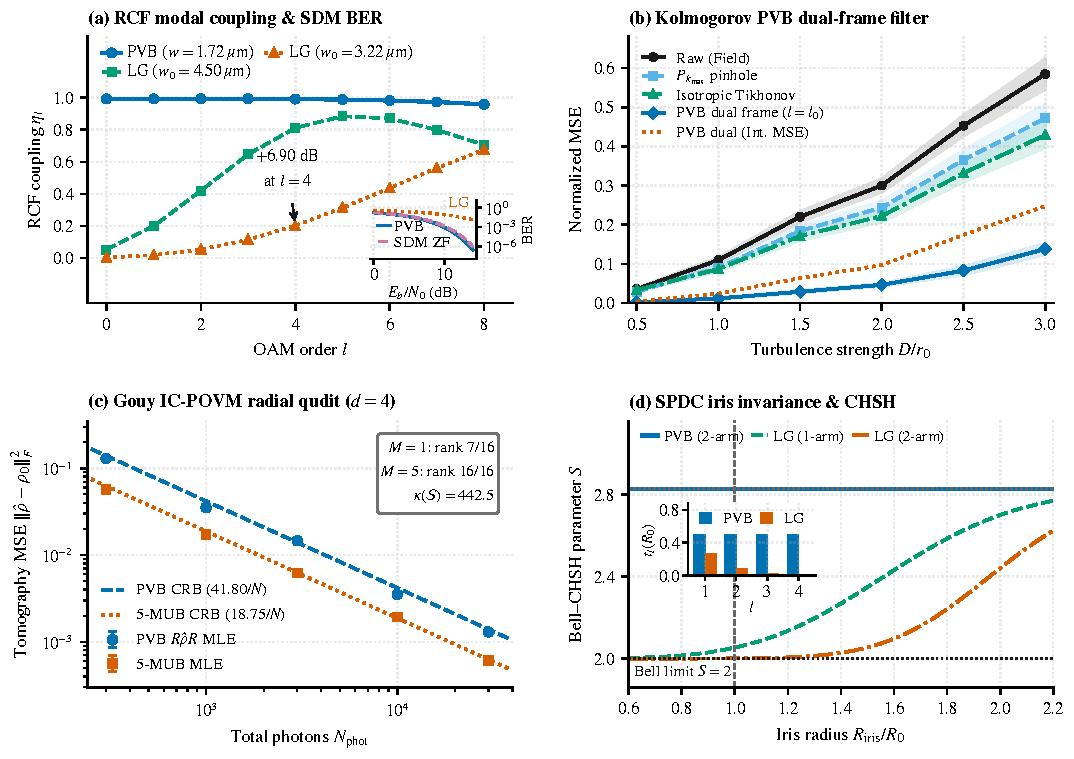
\includegraphics[width=0.82\textwidth]{figures/fig3_optics_utility.pdf}
\caption{Classical and quantum optical utility of PVB continuous and discrete frames. (a) Step-index Sturm--Liouville RCF coupling efficiency $\eta_l$ ($r_1 = 6.0\,\mu\mathrm{m}$, $r_2 = 9.0\,\mu\mathrm{m}$, $n_{\mathrm{clad}} = 1.444$, $\Delta n = 0.033$, $\lambda = 1550\,\mathrm{nm}$) for physical PVBs ($w = 1.72\,\mu\mathrm{m}$, mean $0.985$) versus $\mathrm{LG}_{0,l}$ at channel-matched ($w_0 = 4.50\,\mu\mathrm{m}$) and fixed-collimator ($w_0 = 3.22\,\mu\mathrm{m}$) waists ($+6.90\,\mathrm{dB}$ gain at $l = 4$); inset shows dispersion-free $l = 4$ OOK BER versus pre-coupling $E_b/N_0$ (dB) including the $0.41\,\mathrm{dB}$ ($N = 6$) AWGN ZF penalty at $\Delta R = 2.0\,w$. (b) Normalized field MSE ($\pm 1\,\mathrm{SEM}$) across $40$ subharmonic-corrected Kolmogorov phase screens ($D_{\mathrm{ap}} = 3.0\,\mathrm{mm}$, $z = 0.5\,\mathrm{m}$) comparing raw distortion, circular pinhole $P_{k_{\max}}$, isotropic Tikhonov ($\alpha_{\mathrm{reg}} = 0.0183$), and the single-OAM discrete radial PVB dual-frame projector ($l_0 = 1, N = 5$), alongside PVB dual-frame intensity MSE (dotted). (c) Passive $M = 5$ Gouy-diverse IC-POVM radial-qudit tomography ($d = 4$, $l = 1$, $w/w_0 = 0.25$, full rank $16/16$ versus $7/16$ at $M = 1$, superoperator condition number $\kappa(\mathcal{S}) = 442.5$): $30$-trial $R\hat{\rho}R$ MLE MSE tracks the single-photon CRB $41.80/N_{\mathrm{phot}}$ alongside sequential $5$-MUB tomography ($18.75/N_{\mathrm{phot}}$). (d) Post-selected SPDC Bell--CHSH parameter $S$ versus circular-iris radius $R_{\mathrm{iris}}/R_0$ for $\ket{\Psi} = (\ket{1,-1}+\ket{4,-4})/\sqrt{2}$ ($w = 0.1\,R_0$, LG $w_0 = \sqrt{2}\,R_0$); inset compares single-mode transmissions $t_{1..4}(R_0)$.}
\label{fig:optics_utility}
\end{figure*}

\paragraph*{Single-OAM discrete PVB dual-frame filtering in Kolmogorov turbulence.}
Atmospheric refractive-index fluctuations scatter structured beams into high-$k_\perp$ speckles and neighboring OAM channels~\cite{Paterson2005,TylerBoyd2009,AndrewsPhillips2005}. Importantly, applying only the circular Paley--Wiener pinhole $P_{k_{\max}}$ or the rotationally symmetric Tikhonov filter $S_{w,\alpha_{\mathrm{reg}}}^{-1}S_w$ ($\alpha_{\mathrm{reg}} = e^{-(w k_{\max})^2} = 0.0183$) leaves low-order non-axisymmetric Kolmogorov aberrations (astigmatism, coma) and all azimuthal OAM crosstalk ($l \neq l_0$) unattenuated. To exploit PVB frame structure directly, we project the propagated turbulent field onto the single-OAM discrete radial PVB subspace $\operatorname{span}\{\psi_{l_0,R_n}^{(\mathrm{prop})}\}_{n=1}^N$ ($l_0 = 1$, $N = 5$ concentric rings $R_n \in [0.25, 1.75]\,\mathrm{mm}$ with $\Delta R = 1.5\,w$, $\kappa(\gamma) = 10.12$) using the canonical dual-frame inverse $(\gamma^{-1})_{nm}$ of Proposition~\ref{prop:channel_capacity}:
\begin{equation}
P_{\mathrm{PVB},l_0}\psi_{\mathrm{turb}} = \sum_{n,m=1}^N (\gamma^{-1})_{nm}\braket{\psi_{l_0,R_m}^{(\mathrm{prop})}}{\psi_{\mathrm{turb}}}\psi_{l_0,R_n}^{(\mathrm{prop})}.
\label{eq:discrete_pvb_turb_filter}
\end{equation}
Evaluating $40$ subharmonic-corrected $256\times 256$ Kolmogorov phase screens~\cite{Lane1992} ($D_{\mathrm{ap}} = 3.0\,\mathrm{mm}$, $z = 0.5\,\mathrm{m}$, $R_0 = 1.0\,\mathrm{mm}$, $w = 0.25\,\mathrm{mm}$, $k_{\max} = 8.0\,\mathrm{rad/mm}$) across $D/r_0 \in [0.5, 3.0]$, at $D/r_0 = 3.0$ where $44.8\%$ of total beam power scatters outside the $l_0 = 1$ radial-PVB subspace, isotropic $P_{k_{\max}}$ and Tikhonov filtering reduce field MSE modestly from $0.585$ to $0.471$ and $0.429$, whereas the single-OAM PVB dual-frame projector~\eqref{eq:discrete_pvb_turb_filter} suppresses field MSE by $4.24\times$ to $0.138$ (and intensity MSE from $0.553$ to $0.248$) by simultaneously rejecting all $l \neq l_0$ crosstalk and radial speckle [Fig.~\ref{fig:optics_utility}(b)].

\subsection{Quantum Photonics: Multi-Plane IC-POVM Tomography and Iris Invariance}
\label{subsec:quantum_utility}

\paragraph*{Passive multi-plane Gouy-diverse IC-POVM radial-qudit tomography.}
Consider quantum state tomography on a $d$-dimensional fixed-$l$ radial qudit space $\mathcal{H}_d^{(l)} = \operatorname{span}\{\ket{\psi_{p,l}}\}_{p=0}^{d-1}$. Single-plane ($z = 0$) PVB intensity measurements are \emph{not} informationally complete (IC): because $c_{l,p}(R) \in \mathbb{R}$, single-plane projectors span only $2d - 1 < d^2$ real Hermitian parameters (operator rank $7/16$ at $d = 4$). We lift this real-polynomial degeneracy passively by splitting the beam across $M \ge d+1$ propagation planes $z_m$ (realizable in a single shot via a multi-plane light converter or beam-splitter tree~\cite{Fontaine2019,Bouchard2018}) with distinct Gouy phases $\vartheta_m = \arctan(z_m/z_R)$, where $z_R = k_0 w_0^2/2$. Because at plane $z_m \neq 0$ each $\mathrm{LG}_{p,l}$ state expands in waist by $\sigma_m = \sqrt{1 + (z_m/z_R)^2}$ and acquires spherical wavefront radius $R_c(z_m) = z_m[1 + (z_R/z_m)^2]$, each plane-$z_m$ PVB projector is radially rescaled as $(R_{m,k}, w_m) = \sigma_m(R_k, w)$ and wavefront-matched by a thin compensating lens of focal length $f_m = R_c(z_m)$, defining $\phi_{m,k}(r,\phi) = \sigma_m^{-1} e^{ik_0 r^2/[2R_c(z_m)]}\,\Phi_{l,\sigma_m R_k}(r,\phi;\,\sigma_m w)$. Changing integration variables $r' = r/\sigma_m$ yields the exact POVM elements~\cite{Renes2004}
\begin{align}
\Pi_{m,k} &= \frac{R_k \Delta R}{M}\ket{\phi_{m,k}}\bra{\phi_{m,k}}, \nonumber \\
\braket{\psi_{p,l}(z_m)}{\phi_{m,k}} &= e^{-i(2p+\abs{l}+1)\vartheta_m} c_{l,p}(R_k),
\label{eq:ic_povm_elements}
\end{align}
completed on $\mathcal{H}_d^{(l)}$ by $\Pi_{\mathrm{res}} = I_d - \sum_{m,k}\Pi_{m,k}$ ($\lambda_{\max}(\sum \Pi_{m,k}) = 0.9050 < 1$). For $d = 4$ ($d^2 = 16$), $l = 1$, $w/w_0 = 0.25$, $M = 5$ ($\vartheta_m \in [0, 0.45\pi]$), and $40$ midpoint bins $R_k \in (0, 3.5\,w_0]$, Eq.~\eqref{eq:ic_povm_elements} achieves full IC rank $16/16$, bounded operator-frame condition numbers $\kappa(\mathcal{S}_{\mathrm{POVM}}) = 442.5$ on $\mathrm{Herm}(\mathcal{H}_4)$ and $\kappa_{\mathrm{Bloch}}(\mathcal{S}_{\mathrm{POVM}}) = 88.3$ on the $15$-dimensional traceless Bloch subspace, Fisher condition number $\kappa(\mathbf{F}) = 14.86$ ($\lambda_{\min}(\mathbf{F}) = 0.1261$), and single-photon Cram\'er--Rao bound (CRB) at $\rho_0 = I_4/4$:
\begin{equation}
\operatorname{Tr}\!\left(\mathbf{F}^{-1}\right) = 41.80 \quad (\text{with }\Pi_{\mathrm{res}};\; 42.96\text{ without}),
\label{eq:fisher_crb}
\end{equation}
compared against $18.75$ for $5$ sequential mutually unbiased bases (MUBs), trading a $2.23\times$ photon-budget factor for completely passive, reconfiguration-free single-shot acquisition. Thirty-trial iterative $R\hat{\rho}R$ maximum-likelihood estimation (MLE)~\cite{Lvovsky2004} converges cleanly to $41.80/N_{\mathrm{phot}}$ [Fig.~\ref{fig:optics_utility}(c)].

\paragraph*{$l$-invariant QKD footprint and SPDC circular-iris Bell--CHSH preservation.}
In high-dimensional QKD and spontaneous parametric down-conversion (SPDC)~\cite{Cerf2002,LawEberly2004,Walborn2010,Mirhosseini2015}, a circular pupil $\hat{T}_{\mathrm{iris}} = \Theta(R_{\mathrm{iris}} - r)$ attenuates single-mode $\mathrm{LG}_{0,l}$ detection probabilities as $t_l^{\mathrm{LG}}(R_{\mathrm{iris}}) = \braket{\psi_{0,l}}{\hat{T}_{\mathrm{iris}}\psi_{0,l}} = P(\abs{l}+1, 2R_{\mathrm{iris}}^2/w_0^2)$, creating $l$-dependent efficiency side-channels. By contrast, unit-normalized physical PVBs preserve leading-order $l$-invariant pupil transmission $t_l^{\mathrm{PVB}}(R_{\mathrm{iris}}) = \braket{\psi_{l,R_0}}{\hat{T}_{\mathrm{iris}}\psi_{l,R_0}}$: at $R_{\mathrm{iris}} = R_0$ with $w = 0.1\,R_0$ (versus peak-matched $\mathrm{LG}_{0,l}$ with $w_0 = \sqrt{2}\,R_0$), exact quadrature gives $t_{1..4}^{\mathrm{PVB}} = [0.4999, 0.4996, 0.4991, 0.4984]$ versus $t_{1..4}^{\mathrm{LG}} = [0.2642, 0.0803, 0.0190, 0.0037]$ [Fig.~\ref{fig:optics_utility}(d) inset]. For the two-photon OAM Bell state $\ket{\Psi} = (\ket{1,-1} + \ket{4,-4})/\sqrt{2}$, post-selected single-mode projection through circular irises yields the Bell--CHSH parameter~\cite{Clauser1969}
\begin{equation}
S(R_{\mathrm{iris}}) = 2\sqrt{1 + \mathcal{V}^2(R_{\mathrm{iris}})}, \qquad \mathcal{V} = \frac{2\sqrt{t_1 t_4}}{t_1 + t_4},
\label{eq:iris_chsh}
\end{equation}
for one-arm truncation (with $t_l \mapsto t_l^2$ for symmetric two-arm irises). At $R_{\mathrm{iris}} = R_0$, PVBs retain near-maximal violation $S_{\mathrm{PVB}} = 2.8284$ (two-arm, protected to leading order up to $\mathcal{O}(\Delta r_{\mathrm{peak}}/w)$), whereas $\mathrm{LG}$ modes degrade to $S_{\mathrm{LG}} = 2.0532$ (one-arm) and $2.0008$ (two-arm) [Fig.~\ref{fig:optics_utility}(d)].

\section{Human--AI Collaborative Methodology and Epistemic Governance}
\label{sec:ai_methodology}

\subsection{Generative AI in Theoretical Physics: Cognitive Affordances and Ethical Boundaries}
\label{subsec:ai_ethics}

Scientific methodology in theoretical and computational physics is undergoing a structural shift from purely imperative numerical execution—where software evaluates pre-derived differential equations or quadratures—toward interactive symbolic-and-computational collaboration with large reasoning models~\cite{Wang2023NatureAI,OToole2024,VillaescusaNavarro2025}. Used judiciously, generative AI systems act as high-throughput mathematical assistants capable of testing integral-transform ansatzes, expanding multi-parameter asymptotic series, generating deterministic numerical verification suites, and standardizing technical typesetting~\cite{Haber2025,Jauhiainen2026}. By offloading repetitive symbolic algebra and transcription-heavy coding, such tools allow a human principal investigator to concentrate cognitive effort on physical problem formulation, conceptual unification, and rigorous boundary-condition analysis.

At the same time, recent epistemological and empirical studies demonstrate why unconstrained AI autonomy is incompatible with scientific integrity. Messeri and Crockett~\cite{Messeri2024} warn that uncritical reliance on generative tools fosters ``illusions of explanatory depth,'' while the theoretical-physics benchmark \emph{TheoPhysEval}~\cite{Chandra2026TheoPhysEval} documents systematic failure modes in autonomous derivations: (i) algebraic ``speedruns'' that assert plausible closed forms while bypassing domain, measurability, or convergence hypotheses; (ii) unphysical boundary idealizations (such as substituting singular Dirac rings where finite wavepacket widths govern stability); and (iii) bibliographic fabrication of citations or DOIs~\cite{Kacena2024}. Consistent with editorial policies of the American Physical Society (APS), \emph{Science}~\cite{Thorp2023Science}, and the Committee on Publication Ethics (COPE)~\cite{COPE2023AI}, generative AI cannot bear epistemic or moral responsibility and therefore cannot be an author. Ethical deployment requires a transparent Human-in-the-Loop (HITL) architecture in which the human scientist originates the physical hypotheses, interrogates every intermediate step, and validates all claims deterministically.

\subsection{Collaborative Architecture and Verification Protocol}
\label{subsec:ai_architecture}

The present work was executed through a structured collaboration between the human author (S.~Ayala) and the generative reasoning model Gemini~4~Argon (Google DeepMind) operating within the Antigravity integrated development environment (IDE). To ensure complete mathematical and bibliographic reliability, the workflow enforced a strict separation between human epistemic authority and machine execution across three verification gates:
\begin{enumerate}
\item \emph{Human problem origination and domain specification:} All physical questions, Hilbert-space domains ($L^2(\mathbb{R}^2)$ versus $\mathcal{H}_{k_{\max}}$), frame-versus-state normalization conventions, and optical benchmark regimes were defined and constrained by the human investigator.
\item \emph{Dual symbolic--numerical cross-examination:} No AI-assisted analytical expression was accepted on symbolic plausibility alone; every identity in Secs.~\ref{sec:pvb_formation}--\ref{sec:optics_utility} and Appendix~\ref{app:lg_expansion} was required to agree with independent arbitrary-precision quadrature (\texttt{SciPy}/\texttt{mpmath}) or 2D-FFT/Monte Carlo simulation to machine precision ($\le 10^{-12}$ for exact integrals).
\item \emph{Primary-source bibliographic verification:} Every cited equation number (such as Gradshteyn--Ryzhik formulas 6.631.1 and 6.633.2~\cite{Gradshteyn2014}), experimental fiber parameter~\cite{Villalba2023}, and DOI in the bibliography was verified directly against published records.
\end{enumerate}

\subsection{Concrete Workflow Example: Extending Recent Literature to Arbitrary Radial Order}
\label{subsec:ai_case_study}

A concrete example from this project illustrates how human scientific creativity and critical skepticism interact with AI-accelerated calculation. Starting from two recent studies—Appendix~D of Ferreira \emph{et al.}~\cite{Ferreira2026}, which evaluated the finite-width PVB overlap only for zero-node modes ($p = 0$), and the RCF transmission experiments of Villalba \emph{et al.}~\cite{Villalba2023}—the human investigator posed the guiding creative questions of this manuscript: \emph{Can the $p = 0$ projection in Ref.~\cite{Ferreira2026} be generalized to an exact finite algebraic expansion for all multi-ring $\mathrm{LG}_{p,l}$ modes ($p \ge 1$), how does its continuous frame inverse behave under finite numerical aperture and noise, and why do discrete radial PVB channels remain stable in practice despite continuous radial overlap?}

During interactive exploration, critical questioning by the human physicist exposed and corrected three subtle pitfalls in preliminary AI derivations:
\begin{enumerate}
\item \emph{Separating frame scaling from state normalization:} An unguarded discrete Gram calculation using the frame elements $\Phi_{l,R}$ predicted a spuriously diverging condition number $\kappa(G) = 80.02$ at $N = 120$ rings. Questioning why physically decoupled outer rings could degrade conditioning led the human author to isolate the $R^{-1}$ norm decay of $\norm{\Phi_{l,R}}_{L^2}^2$ and formulate Proposition~\ref{prop:channel_capacity} in terms of the unit-normalized matrix $\gamma_{nm}$ ($\kappa(\gamma) = 1.741$), alongside the explicit Convention of Sec.~\ref{subsec:pvb_def} and Lemma~\ref{lem:bessel_upper}.
\item \emph{Resolving unbounded $L^2$ inversion and propagation physics:} Formal inversion of $\widetilde{G}_w(k_\perp) = e^{-w^2 k_\perp^2/2}$ initially overlooked that $S_w^{-1}\Phi_{l,R} \notin L^2(\mathbb{R}^2)$, and an initial propagation remark conflated pre-focal axicon self-healing ($k_0 R/k_r = f$) with post-focal Fresnel diffraction. Human physical auditing enforced the Paley--Wiener restriction $S_{w,k_{\max}} = P_{k_{\max}}S_w P_{k_{\max}}\big|_{\mathcal{H}_{k_{\max}}}$ in Theorem~\ref{thm:pw_bounds}, the explicit Fourier-annulus sharpness proof~\eqref{eq:sharpness_limits}, and the two-zone propagation physics of Remark~\ref{rem:propagation}.
\item \emph{Exploiting genuine frame selectivity in turbulence and Gouy tomography:} Recognizing that isotropic Fourier filters cannot reject $l \neq l_0$ OAM crosstalk and that $z_m \neq 0$ Gouy planes carry beam expansion $\sigma_m$ and curvature $R_c(z_m)$, the human author redirected the turbulence benchmark to the single-OAM discrete PVB dual-frame projector~\eqref{eq:discrete_pvb_turb_filter} and incorporated explicit lens/waist matching into Eq.~\eqref{eq:ic_povm_elements}.
\end{enumerate}
Once these physical guardrails were established, delegating the Kummer hypergeometric summation algebra in Appendix~\ref{app:lg_expansion}, the 60-entry 50-digit quadrature verification harness (Table~\ref{tab:c_lp_verification}), and multi-panel vector figure scripting to Gemini~4~Argon substantially reduced the time spent on repetitive, error-prone manipulations—demonstrating an efficient, verifiable, and ethically transparent model for human--AI theoretical physics.

\section{Conclusions}
\label{sec:conclusions}

Addressing the four questions posed in Sec.~\ref{sec:intro}, we have established a rigorous operator-theoretic foundation for finite-width physical PVBs as continuous Hilbert frames. While azimuthal OAM sectors decouple into strictly orthogonal subspaces ($\mathcal{H} = \bigoplus_{l\in\mathbb{Z}}\mathcal{H}_l$), finite ring half-width $w > 0$ induces an isotropic Gaussian convolution frame operator $S_w = G_w * \cdot$ with optimal Bessel upper bound $B = 1$, vanishing global lower bound $A = 0$ on unconstrained $L^2(\mathbb{R}^2)$, and sharp Paley--Wiener stability bounds $A = \exp(-w^2 k_{\max}^2/2)$ and $B = 1$ on $\mathcal{H}_{k_{\max}}$ (Lemma~\ref{lem:bessel_upper}, Proposition~\ref{prop:conv_kernel}, and Theorem~\ref{thm:pw_bounds}). Building on this structure, we constructed the Tikhonov-regularized canonical dual frame and proved its noise-gain peak $(2\sqrt{\alpha_{\mathrm{reg}}})^{-1}$ at $k_{\mathrm{peak}} = w^{-1}\sqrt{\ln(1/\alpha_{\mathrm{reg}})}$ (Proposition~\ref{prop:tikhonov_dual}), derived the exact $(p+1)$-term closed-form expansion $c_{l,p}(R)$ for all $\mathrm{LG}_{p,l}$ modes ($p \ge 0$, Theorem~\ref{thm:c_lp_exact}), established both the exact $p = 0$ threshold and the generalized radial Rayleigh limit $w_{\mathrm{crit}} \approx 0.573\,w_0/\sqrt{2p+\abs{l}+1}$ ($p \ge 1$, Corollary~\ref{cor:rayleigh_radial}), and proved monotonic unit-normalized Gram conditioning ($\kappa(\gamma) = 1.645$ and $17.36\,\mathrm{dB}$ isolation at $\Delta R = 2.0\,w$, Proposition~\ref{prop:channel_capacity}).

Across classical and quantum photonics, these frame properties translate directly into $258.6\times$ regularized noisy reconstruction gain, $>98.5\%$ mean RCF coupling with $<0.42\,\mathrm{dB}$ multi-ring equalization penalty, $4.24\times$ Kolmogorov field-MSE suppression via single-OAM discrete PVB dual-frame projection, reconfiguration-free $M = 5$ Gouy-diverse radial-qudit IC-POVM tomography (rank $16/16$), and leading-order circular-iris Bell--CHSH entanglement protection. Finally, our documented HITL workflow illustrates how human physical intuition and adversarial auditing can be paired ethically with generative reasoning tools to accelerate exact analytical and computational physics.

\begin{acknowledgments}
AI disclosure: Portions of this work were developed in collaboration with Gemini~4~Argon (Google DeepMind) operating within the Antigravity IDE (accessed November 2026), which assisted with symbolic integral transformations, asymptotic series checks, reproducible Python verification and plotting scripts, and \LaTeX{} typesetting as detailed in Sec.~\ref{sec:ai_methodology}. All research questions, physical hypotheses, mathematical domain specifications, analytical audits, and scientific conclusions were conceived and verified by the sole human author, Sebasti\'an Ayala, who assumes full responsibility for the integrity and accuracy of the manuscript in accordance with American Physical Society editorial policies.
\end{acknowledgments}

\section*{Data Availability}
All analytical verification scripts, first-principles optical simulation routines (\texttt{pvb\_\allowbreak physics.py}, \texttt{verify\_\allowbreak analytical\_\allowbreak tables.py}, and \texttt{generate\_\allowbreak figures\_\allowbreak and\_\allowbreak metrics.py}), and machine-precision numerical benchmark datasets supporting the findings of this study are self-contained and openly available from the author upon reasonable request and in the accompanying open-source code distribution.

\appendix
\section{Derivation and Quadrature Verification of the Closed-Form \texorpdfstring{$\mathrm{LG}_{p,l}$}{LG\_\{p,l\}} Expansion}
\label{app:lg_expansion}

Evaluating $c_{l,p}(R) = \braket{\Phi_{l,R}}{\psi_{p,l}}$ from Eqs.~\eqref{eq:pvb_mode} and~\eqref{eq:lg_def} and integrating over the azimuthal angle $\phi \in [0,2\pi)$ gives
\begin{align}
c_{l,p}(R) &= 2\pi C_0 N_{p,l} e^{-R^2/w^2} \int_0^\infty r\,dr\, e^{-a_0 r^2} I_{\abs{l}}(b_R r) \nonumber \\
&\quad \times \left(\frac{\sqrt{2}\,r}{w_0}\right)^{\abs{l}} L_p^{\abs{l}}\!\left(\frac{2r^2}{w_0^2}\right),
\label{eq:app_c_int}
\end{align}
where $a_0 = 1/w^2 + 1/w_0^2 = (w_0^2+w^2)/(w^2 w_0^2)$, $b_R = 2R/w^2$, $N_{p,l} = \sqrt{2p!/[\pi(p+\abs{l})!]}/w_0$, and we used $I_l(b_R r) = I_{\abs{l}}(b_R r)$ for $l \in \mathbb{Z}$.

Before treating general $p \ge 0$, we verify the fundamental $p = 0$ limit directly via Weber's exponential integral. For $p = 0$ and $l = 0$, $L_0^0 \equiv 1$ and $N_{0,0} = \sqrt{2/\pi}/w_0$, so Eq.~\eqref{eq:app_c_int} reduces to
\begin{align}
c_{0,0}(R) &= \frac{4}{w^2 w_0} e^{-R^2/w^2} \int_0^\infty r\,e^{-a_0 r^2} I_0(b_R r)\,dr \nonumber \\
&= \frac{4}{w^2 w_0} e^{-R^2/w^2} \frac{1}{2a_0} \exp\!\left(\frac{b_R^2}{4a_0}\right) \nonumber \\
&= \frac{2w_0}{w_0^2 + w^2} \exp\!\left(-\frac{R^2}{w_0^2 + w^2}\right) = \mathcal{A}_{0,0}(R),
\label{eq:app_p0_l0_check}
\end{align}
since $-R^2/w^2 + b_R^2/(4a_0) = -R^2/(w_0^2 + w^2)$. More generally, at $p = 0$ and any $l \in \mathbb{Z}$, $L_0^{\abs{l}} \equiv 1$ and Gradshteyn--Ryzhik formula 6.631.4~\cite{Gradshteyn2014} gives $\int_0^\infty r^{\abs{l}+1} e^{-a_0 r^2} I_{\abs{l}}(b_R r)\,dr = b_R^{\abs{l}} (2 a_0)^{-\abs{l}-1} e^{b_R^2/(4a_0)}$, reproducing $c_{l,0}(R) = \mathcal{A}_{0,l}(R)$ in exact agreement with Ref.~\cite{Ferreira2026} up to the unit-norm factor $\norm{\Phi_{l,R}}_{L^2}^{-1}$.

For arbitrary $p \ge 0$, expanding the associated Laguerre polynomial $L_p^{\abs{l}}(2r^2/w_0^2) = \sum_{m=0}^p (-1)^m \allowbreak \binom{p+\abs{l}}{p-m} \allowbreak (m!)^{-1} \allowbreak (2/w_0^2)^m r^{2m}$ [equivalently extracted from the generating function $(1-t)^{-\abs{l}-1}\allowbreak \exp[-2r^2 t/(w_0^2(1-t))] = \sum_{p=0}^\infty t^p L_p^{\abs{l}}(2r^2/w_0^2)$] separates Eq.~\eqref{eq:app_c_int} into $(p+1)$ radial integrals:
\begin{align}
\mathcal{J}_{p,l} &= \left(\frac{\sqrt{2}}{w_0}\right)^{\abs{l}} \sum_{m=0}^p \frac{(-1)^m}{m!}\binom{p+\abs{l}}{p-m}\left(\frac{2}{w_0^2}\right)^m \nonumber \\
&\quad \times \int_0^\infty r^{\abs{l}+2m+1} e^{-a_0 r^2} I_{\abs{l}}(b_R r)\,dr.
\label{eq:app_J_sum}
\end{align}
Each integral in Eq.~\eqref{eq:app_J_sum} closes via formula 6.631.1 of Gradshteyn and Ryzhik~\cite{Gradshteyn2014}, analytically continued via $J_\nu(i b_R r) = i^\nu I_\nu(b_R r)$ for $\operatorname{Re}(a_0) > 0$ and $\operatorname{Re}(\mu+\nu) > 0$:
\begin{align*}
\int_0^\infty r^{\mu-1} e^{-a_0 r^2} I_\nu(b_R r)\,dr &= \frac{b_R^\nu\,\Gamma\!\left(\frac{\mu+\nu}{2}\right)}{2^{\nu+1} a_0^{(\mu+\nu)/2}\Gamma(\nu+1)} \\
&\quad \times {_1F_1}\!\left(\frac{\mu+\nu}{2}; \nu+1; \frac{b_R^2}{4a_0}\right).
\end{align*}
Setting $\nu = \abs{l} \ge 0$ and $\mu = \abs{l} + 2m + 2$ gives $(\mu+\nu)/2 = \abs{l} + m + 1$, yielding
\begin{align}
&\int_0^\infty r^{\abs{l}+2m+1} e^{-a_0 r^2} I_{\abs{l}}(b_R r)\,dr \nonumber \\
&\quad = \frac{b_R^{\abs{l}}(\abs{l}+m)!}{2^{\abs{l}+1} a_0^{\abs{l}+m+1}\abs{l}!}\,{_1F_1}\!\left(\abs{l}+m+1; \abs{l}+1; \zeta_R\right),
\label{eq:app_hypergeom}
\end{align}
where $\zeta_R = b_R^2/(4a_0) = R^2 w_0^2/[w^2(w_0^2+w^2)]$. Applying Kummer's first transformation ${_1F_1}(a;b;\zeta_R) = e^{\zeta_R}\,{_1F_1}(b-a;b;-\zeta_R)$ to Eq.~\eqref{eq:app_hypergeom} sets $b - a = -m$, terminating the hypergeometric series as an associated Laguerre polynomial of degree $m$:
\begin{equation}
{_1F_1}\!\left(-m; \abs{l}+1; -\zeta_R\right) = \frac{m!\,\abs{l}!}{(\abs{l}+m)!}\,L_m^{\abs{l}}(-\zeta_R).
\label{eq:app_kummer_laguerre}
\end{equation}
Canceling the factorials $m!$, $\abs{l}!$, and $(\abs{l}+m)!$ between Eqs.~\eqref{eq:app_J_sum}--\eqref{eq:app_kummer_laguerre}, identifying $[2/(a_0 w_0^2)]^m = \xi^m$, and collecting $2\pi C_0 N_{p,l} b_R^{\abs{l}} 2^{-(\abs{l}+1)} a_0^{-(\abs{l}+1)} (\sqrt{2}/w_0)^{\abs{l}} e^{-R^2/w^2 + \zeta_R} = \mathcal{A}_{p,l}(R)$ proves Eqs.~\eqref{eq:c_lp_exact}--\eqref{eq:A_prefactor} of Theorem~\ref{thm:c_lp_exact}. Table~\ref{tab:c_lp_verification} benchmarks Eq.~\eqref{eq:c_lp_exact} against 50-digit numerical quadrature across 60 parameter combinations, confirming $\abs{\Delta c}/\abs{c} \le 3.64\times 10^{-12} \ll 10^{-6}$ throughout.

\begin{table*}[t]
\caption{Numerical verification of the closed-form $\mathrm{LG}_{p,l}$ frame expansion $c_{l,p}(R)$ [Eq.~\eqref{eq:c_lp_exact}] against arbitrary-precision radial quadrature of Eq.~\eqref{eq:app_c_int} across $(p,l) \in \{(0,0),(1,0),(0,1),(2,1),(3,2)\}$, $w/w_0 \in \{0.25, 0.50, 1.00\}$, and $R/w_0 \in \{0.5, 1.0, 1.5, 2.0\}$ ($w_0 = 1$, 60 total entries). Closed-form and quadrature values agree identically to all six displayed significant digits; the rightmost column reports the maximum IEEE-754 relative discrepancy $\max_R \abs{c_{\mathrm{exact}} - c_{\mathrm{quad}}}/\abs{c_{\mathrm{quad}}}$ across the four radii in each row.}
\label{tab:c_lp_verification}
\begin{ruledtabular}
\footnotesize
\setlength{\tabcolsep}{4pt}
\begin{tabular}{ccrrrrrc}
Mode $(p,l)$ & $w / w_0$ & $c_{l,p}(0.5\,w_0)$ & $c_{l,p}(1.0\,w_0)$ & $c_{l,p}(1.5\,w_0)$ & $c_{l,p}(2.0\,w_0)$ & $\max_R \abs{\Delta c}/\abs{c}$ \\
\hline
$(0,0)$ & $0.25$ & $+1.487696$ & $+0.734435$ & $+0.226474$ & $+0.043622$ & $1.23\times 10^{-16}$ \\
$(0,0)$ & $0.50$ & $+1.309969$ & $+0.718926$ & $+0.264478$ & $+0.065220$ & $1.70\times 10^{-16}$ \\
$(0,0)$ & $1.00$ & $+0.882497$ & $+0.606531$ & $+0.324652$ & $+0.135335$ & $<1.0\times 10^{-16}$ \\
\hline
$(1,0)$ & $0.25$ & $+0.653762$ & $-0.653113$ & $-0.702932$ & $-0.270640$ & $1.70\times 10^{-16}$ \\
$(1,0)$ & $0.50$ & $+0.366791$ & $-0.488870$ & $-0.603010$ & $-0.294792$ & $2.27\times 10^{-16}$ \\
$(1,0)$ & $1.00$ & $-0.110312$ & $-0.303265$ & $-0.365234$ & $-0.270671$ & $<1.0\times 10^{-16}$ \\
\hline
$(0,1)$ & $0.25$ & $+0.990080$ & $+0.977551$ & $+0.452164$ & $+0.116125$ & $2.39\times 10^{-16}$ \\
$(0,1)$ & $0.50$ & $+0.741030$ & $+0.813372$ & $+0.448834$ & $+0.147575$ & $1.50\times 10^{-16}$ \\
$(0,1)$ & $1.00$ & $+0.312010$ & $+0.428882$ & $+0.344346$ & $+0.191393$ & $1.78\times 10^{-16}$ \\
\hline
$(2,1)$ & $0.25$ & $+0.721001$ & $-0.442836$ & $-0.070805$ & $+0.582387$ & $4.12\times 10^{-15}$ \\
$(2,1)$ & $0.50$ & $+0.237534$ & $-0.190094$ & $+0.011195$ & $+0.423558$ & $2.77\times 10^{-14}$ \\
$(2,1)$ & $1.00$ & $+0.001407$ & $+0.030952$ & $+0.125808$ & $+0.221002$ & $3.08\times 10^{-16}$ \\
\hline
$(3,2)$ & $0.25$ & $+0.565705$ & $-0.269604$ & $+0.066491$ & $+0.218546$ & $2.28\times 10^{-14}$ \\
$(3,2)$ & $0.50$ & $+0.108369$ & $-0.069946$ & $+0.042970$ & $+0.050772$ & $2.84\times 10^{-14}$ \\
$(3,2)$ & $1.00$ & $-8.02947\times 10^{-6}$ & $-0.001413$ & $-0.019380$ & $-0.080698$ & $3.64\times 10^{-12}$ \\
\end{tabular}
\end{ruledtabular}
\end{table*}

\bibliography{references}

\end{document}
